%----------------------------------------------------------------------------
\chapter{\SystemDesign}
%----------------------------------------------------------------------------
\section{Követelmények}
%----------------------------------------------------------------------------
Az új rendszer tervezésekor a következő szempontokat kellett szem előtt tartanom:
\begin{itemize}
	\item Teljesen digitális megoldás kialakítása.
	\item Redundáns rendszer kialakítása biztosítva a folyamatos működést.
	\item Rugalmas felépítés, amely lehetővé teszi a könnyű alkalmazkodást változó körülményekhez.
	\item Könnyen bővíthető struktúra kialakítása a jövőbeli igényekhez való gyors reagálás érdekében.
	\item Magasabb hangminőség és hangnyomás elérésének lehetősége a korábbi rendszerrel összehasonlítva.
	\item Jobb lefedettség és egyenletes hangvisszaadás biztosítása a közönség területén.
	\item A piacon lévő termékekhez képest viszonylag költséghatékony megoldás kidolgozása.
	\item Legyen hosszú távon egy kompetitív és korszerű rendszer.
	\item Megbízható és kiforrott technológiára épüljön.
\end{itemize}
%----------------------------------------------------------------------------
\section{Rendszerterv}
%----------------------------------------------------------------------------
A szakdolgozatomban megtervezésre kerülő hangrendszer lelke a Dante protokoll lesz.
Hangládák szempontjából a Martin Audio Wavefront Precision szériás termékeire esett a választás.
Mivel teljes mértékben digitális rendszert elérése volt a cél, ezért a Dante modullal
rendelkező Martin Audio iKON iK42 és iK81 végfokok tökéletesen illeszkedtek a rendszerbe.
Mindkét végfok csúcskategóriás teljesítményt és hangminőséget nyújt, és a D kategóriás
erősítőknek köszönhetően rendkívül kis helyet foglalnak el a rack-ben miközben kiváló hatásfok
mellett képesek nagy teljesítményt leadni. A két erősítő között két fundamentális különbség van,
az iK42 négy kimeneti csatornával rendelkezik, 20.000 W teljesítmény leadása mellett. 
Ezzel szemben az iK81 nyolc kimeneti csatornával rendelkezik, 10.000 W teljesítménnyel. \cite{IKONAMPUSEGUIDE}
A végfokokat a Dante hálózaton keresztül fogjuk jellel ellátni, így a hagyományos analóg XLR, vagy AES kábelezés helyett
két CAT5E kábellel (a redundancia miatt) tudjuk a végfokokat a hálózatra kötni. 
A végfokrendszer fő vezérlő protokollja miatt szükség lesz még egy CAT5E alapú
összeköttetésre, ami az egyes végfokokat köti össze egy hálózatba a switcheken keresztül. (VU-NET protokoll)
Minden egyes végfokrackben két MikroTik 24 portos switch lesz. Az egyik switch a Dante elsődleges hálózatát fogja kizárólag kezelni.
A másik switch a Dante másodlagos hálózatát, és a VU-NET hálózatot fogja kezelni.
Ez a két alhálózat VLAN szegmensekkel lesz elkülönítve, hogy a hálózat biztonságos és stabil legyen.
%----------------------------------------------------------------------------
\begin{figure}[H]
    \centering
    \begin{minipage}{0.45\textwidth}
        \centering
        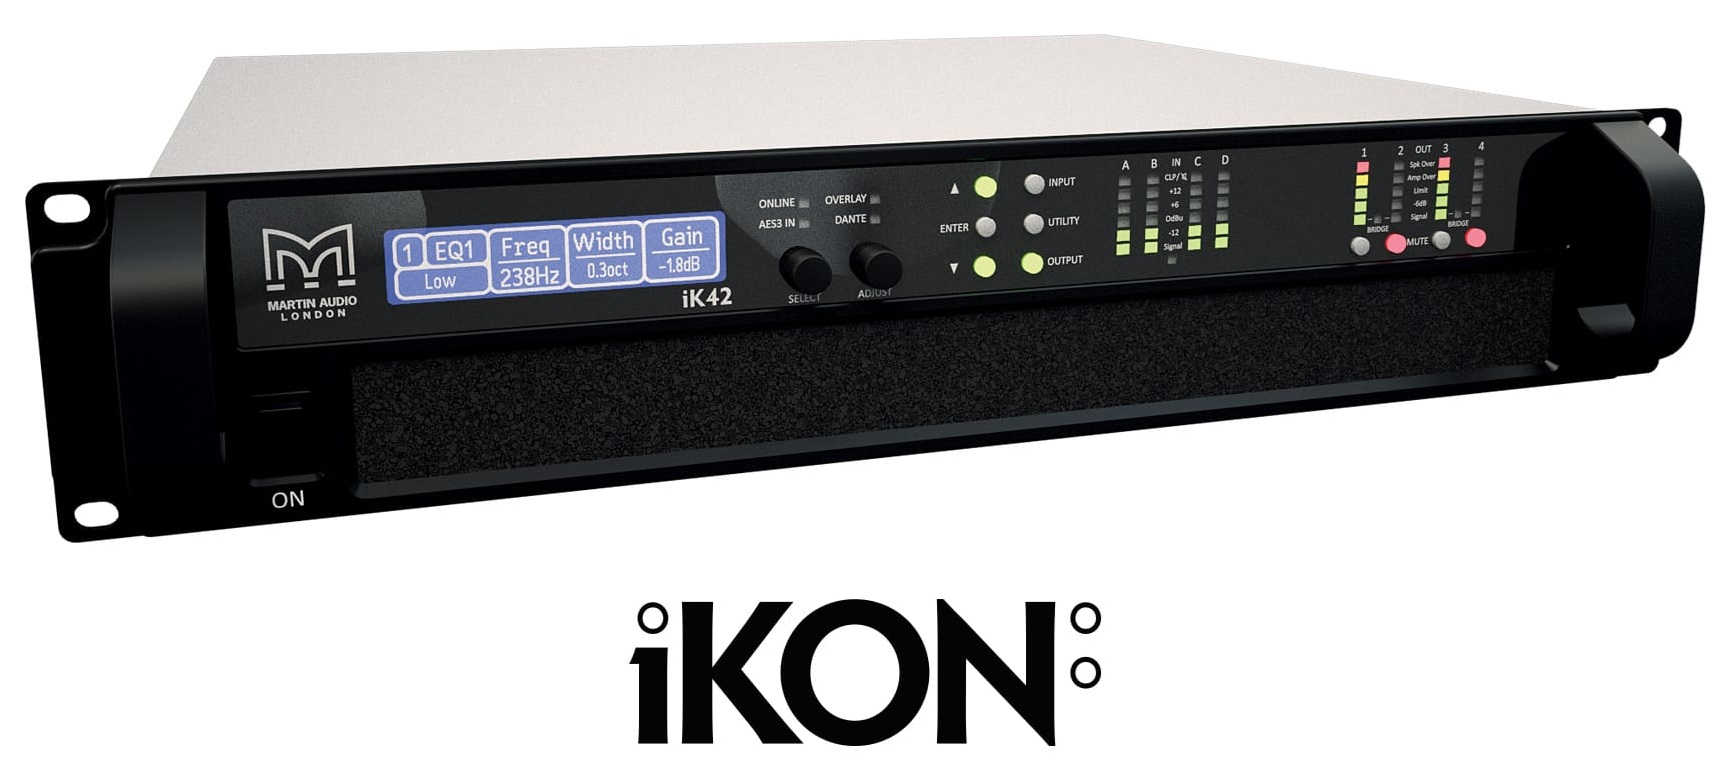
\includegraphics[width=\linewidth, keepaspectratio]{figures/ikon_ik42.jpg}
        \caption{Martin Audio iK42 végfok}\label{fig:ikon_ik42}
    \end{minipage}\hfill
    \begin{minipage}{0.45\textwidth}
        \centering
        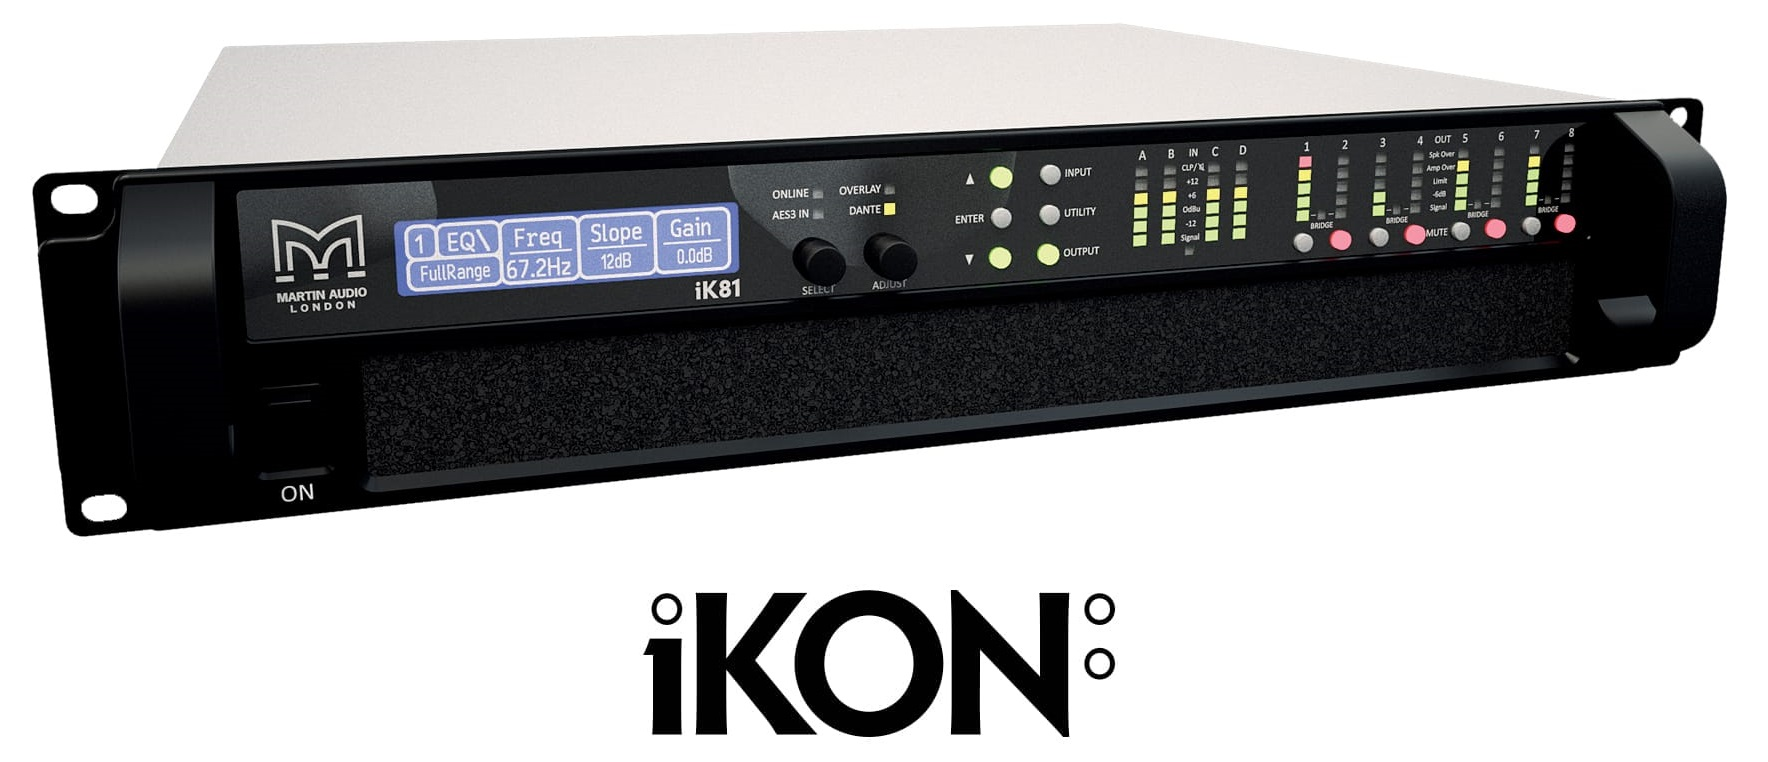
\includegraphics[width=\linewidth, keepaspectratio]{figures/ikon_ik81.jpg}
        \caption{Martin Audio iK81 végfok}\label{fig:ikon_ik81}
    \end{minipage}
\end{figure}
%----------------------------------------------------------------------------

!!!ÁBRA HELYE!!! Egy jel útja a régi hibrid rendszerben

!!!ÁBRA HELYE!!! Egy jel útja az új teljesen digitális rendszerben

%----------------------------------------------------------------------------
\subsection{Martin Audio Wavefront Precision hangrendszer}
%----------------------------------------------------------------------------
\subsubsection{Martin Audio Display 2.3.4 b1 tervező szoftver \cite{DISPLAY23USERGUIDE}}
%----------------------------------------------------------------------------
Mielőtt bele fognánk a tervezési folyamatba, fontos megemlíteni, hogy a szoftver
eredetileg Intel alapú processzorokra lett tervezve és MatLab alapú. Ebből fakadóan
AMD Ryzen processzorokon habár elindult a szoftver, de nem volt stabil és a számítások során
minden esetben összeomlott, és használhatatlanul lassú volt. Személy szerint a saját gépem amivel dolgoztam
sajnos ilyen processzorral van szerelve ezért muszáj volt megoldást találni a problémára.
A Martin Audio hivatalos szoftveres támogatásához fordultam először, de sajnos nem tudtak segíteni.
Ezért a szoftver használatához
sok belefektetett óra olvasás után sikerült egy olyan MatLab CMD parancsot találnom, amivel
a szoftver elindul és használható.
Miután rájöttem a probléma gyökerére, ezt megosztottam velük, hogy a jövőben másoknak ne kelljen
ezzel a problémával szembesülniük.
A hiba az alábbi volt. Az új AMD Ryzen processzorok másfajta utasításkészletet használnak.
Ebből kifolyólag a MatLab 2015-s runtime alapú szoftver adta alaputasításokat nem tudta értelmezni a CPU.
A vezető szoftvermérnökkel való e-mail-es beszélgetésünk során megköszönte a probléma
megoldását, és nemsokkal a megoldásom megosztása után a hivatalos oldalra is felekerült
az indító parancsfájl. Az e-mailben további kollaborációra is adott lehetőséget.
A kompatibilitási problémát rögtön a script elején megoldottam,
mivel a következő parancs megadásával már használhatóvá válik a program: \texttt{set MKL\_DEBUG\_CPU\_TYPE=5} \newline
Ez a sor a program vezérlését AVX2-re állítja át, és mivel ezt az utasításkészletet már ismeri az AMD Ryzen processzor
is ezért a probléma már a múlté.
Az indító fájl további sorai optimalizálások a számítások gyorsítására, és a párhuzamosítására, ezzel jobban kihasználva
a rendelkezésre álló hardver erőforrásokat.
%----------------------------------------------------------------------------
\begin{lstlisting}[caption={A Display 2.3.4 b1 indító ".bat" scriptje AMD Ryzen processzorokhoz}, label=batcode, xleftmargin=\parindent]
    @echo off
    set PATH=%PATH%;C:\Program Files\Martin Audio\Display2_3_4_b1\application
    set MKL_DEBUG_CPU_TYPE=5
    set options=optimoptions('ga','UseParallel',true,'UseVectorized',false)
    set options=optimoptions('gamultiobj','UseParallel',true,'UseVectorized',false)
    set options=optimoptions('paretosearch','UseParallel',true)
    set options=optimoptions('particleswarm','UseParallel',true,'UseVectorized',false)
    set options=optimoptions('patternsearch','UseParallel',true,'UseCompletePoll',true,'UseVectorized',false)
    set options=optimoptions('surrogateopt','UseParallel',true)
    set GPUAcceleration=on
    start "Martin Audio" Display2_3_4_b1.exe
    pause
\end{lstlisting}
%----------------------------------------------------------------------------
\begin{figure}[H]
	\centering
	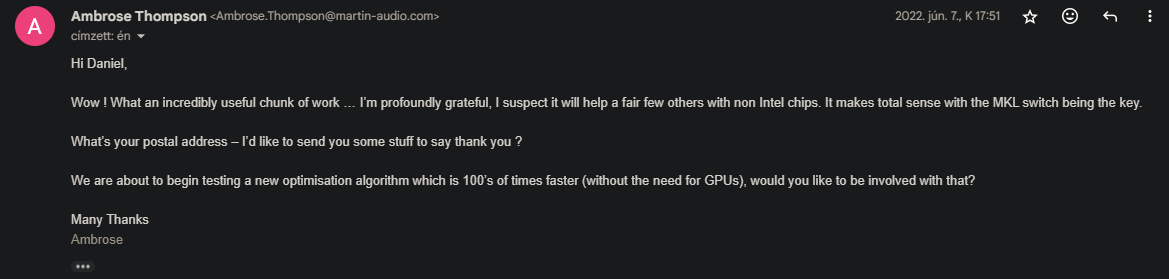
\includegraphics[width=\textwidth, keepaspectratio]{figures/ambrose_email.png}
	\caption{E-mail a Martin Audio vezető szoftvermérnökétől}
	\label{fig:ambrose_email}
\end{figure}
%----------------------------------------------------------------------------
Most, hogy már a szoftver használható és teljes mértékben működőképes, kezdjük el a tervezést.
A modellezés során a budapesti Millenáris B csarnoka lesz a referencia helyszín. Két LineArray rendszert fogunk
tervezni, mivel a terem hosszúsága és a lefedettség növelése miatt szükségünk lesz Delay kiegészítésre a fő hangrendszerhez.
Első lépésben a fő hangrendszert tervezem meg, ami oldalanként (bal és jobb) 8 darab WPC LineArray modulból fog állni.
Ez a láda 2 darab 10"-os mélysugárzót (LF), 2 darab 5"-os közép sugárzót (MF) és 4 darab 0.7"-os magassugárzót tartalmaz (HF).
Három utas Bi-amp meghajtású külső végfokot igénylő rendszer, ahol a mély tartományt (+1,-1) és a középmagas tartományt (+2,-2) külön kezeljük,
a négy pólusú Neutrik Speakon csatlakozókon keresztül.
A láda maximális hangnyomás szintje 135 dB, és 65 Hz-től 18 kHz-ig terjed a frekvencia átvitele +- 3 dB pontossággal. \cite{WPCUSERGUIDE}
%----------------------------------------------------------------------------
\begin{figure}[H]
	\centering
	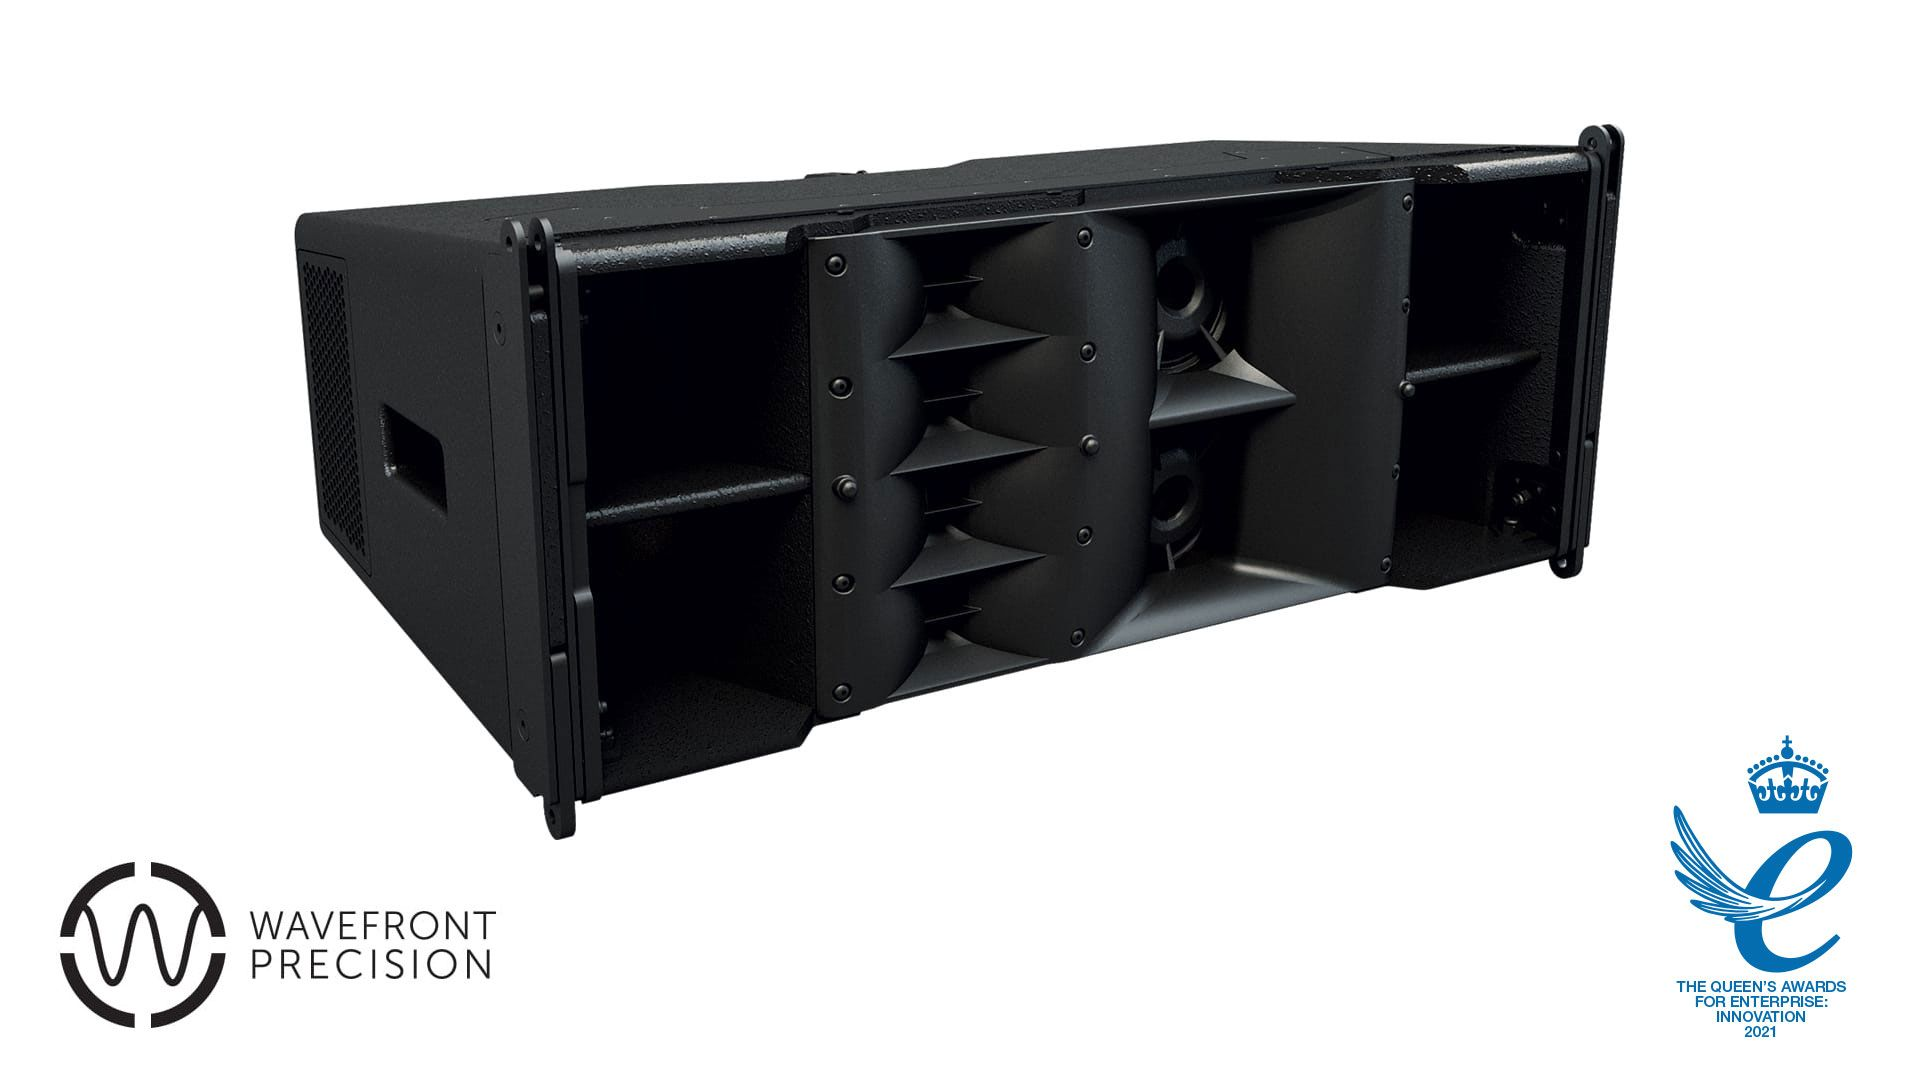
\includegraphics[width=80mm, keepaspectratio]{figures/wpc_front_view.jpg}
	\caption{Martin Audio WPC LineArray modul}\label{fig:wpc}
\end{figure}
%----------------------------------------------------------------------------
A program megnyitásakor a legelső lépés, hogy kiválasztjuk a termékpalettából a megfelelő hangrendszert.
Jelen esetben az előbbiekben említett WPC-t. A produkció igényei, a nagy létszámú közönség és a ládamennyiség miatt a rendszert
\textit{``riggelni''} fogjuk. (maximálisan 6 darab WPC-t lehet \textit{``stackelni''}, azaz a földre vagy mélyládákra helyezni)
A helyszín felmérése után a hangrendszer \textit{``riggelése''} lehetséges, mivel a csarnokban található tartószerkezet biztonságosan
és tartósan képes elviselni a rendszer súlyát.
A telepítés módja kiválasztása után megadjuk a szoftvernek a tervezni való hangláda mennyiséget, ez az esetünkben már említett 8 darab.
A hozzáadás gombra kattintva a elénk kerül a fő kezelőfelület, ahol a hangrendszert tudjuk lépésről lépésre tervezni.
%----------------------------------------------------------------------------
\begin{figure}[H]
	\centering
	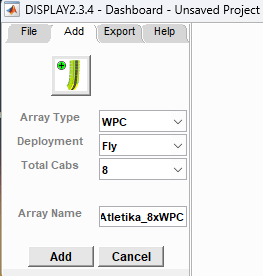
\includegraphics[width=50mm, keepaspectratio]{figures/display_wpc_0.png}
	\caption{Display 2.3.4 b1 kezdőképernyője (WPC)}\label{fig:display_wpc_0}
\end{figure}
%----------------------------------------------------------------------------
A tervezési folyamat öt részre osztható, amiket a szoftverben külön kezelünk.
Ezeket a \textit{``Slice''}, \textit{``Cover''}, \textit{``Splay''}, \textit{``Rig''} és \textit{``EQ''} kezelőfelületeken tudjuk elvégezni,
balról jobbra haladva. Mivel a különböző részegységek egymásra épülnek, ezért fontos a sorrend betartása.
(tervezés utáni módosításokra természetesen van lehetőség, de az adott projekt első tervezési folyamata során ezeket a lépéseket kell követni)
%----------------------------------------------------------------------------
\begin{figure}[H]
	\centering
	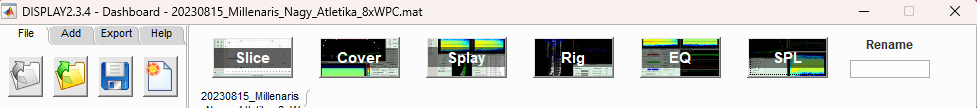
\includegraphics[width=\textwidth, keepaspectratio]{figures/display_wpc_0_1.png}
	\caption{Display 2.3.4 b1 fő kezelőfelülete (WPC)}\label{fig:display_wpc_0_1}
\end{figure}
%----------------------------------------------------------------------------
A \textit{``Slice''} panelen meghatározzuk a rendszer fizikai pozícióját térben. A csarnok
pontos lemodellezése érdekében a mérésekhez lézeres távolságmérőt használtam.
Mivel minden egyes rendezvényen más és más a különböző elemek elhelyezkedése, ezért a
rendszert minden alkalommal újra kell tervezni, még akkor is ha maga a helyszín nem változik.
\textit{``Vertex''} pontok segítségével tudjuk a méreteket és a pozíciókat meghatározni.
A 2D-s modellen figyelembe kell venni a terem önálló méretén kívül a színpadod és a színpad mögötti területet is.
A rajznak tartalmazni kell azokat a falfelületeket is amelyeknél a hangvisszaverődést minimalizálni szeretnénk,
ennek az optimalizáció későbbi fázisában lesz jelentősége.
A terem pontos rajza után még két fontos paramétert kell megadni ezen a felületen.
El kell helyeznünk magát a hangrendszert a teremben, és meg kell határoznunk milyen magasra szeretnénk a rendszert emelni.
Mivel a csarnok rendkívül hosszú, és a adottságai megengedik, ezért a rendszert minél magasabbra szeretnénk emelni,
a jobb lefedettség érdekében.
A másik fontos paraméter az optimalizációhoz, a közönség területének meghatározása. Kezdő és végpont segítségével
tudjuk a területet meghatározni, ahol a hallgatóközönség tartózkodni fog.
%----------------------------------------------------------------------------
\begin{figure}[H]
	\centering
	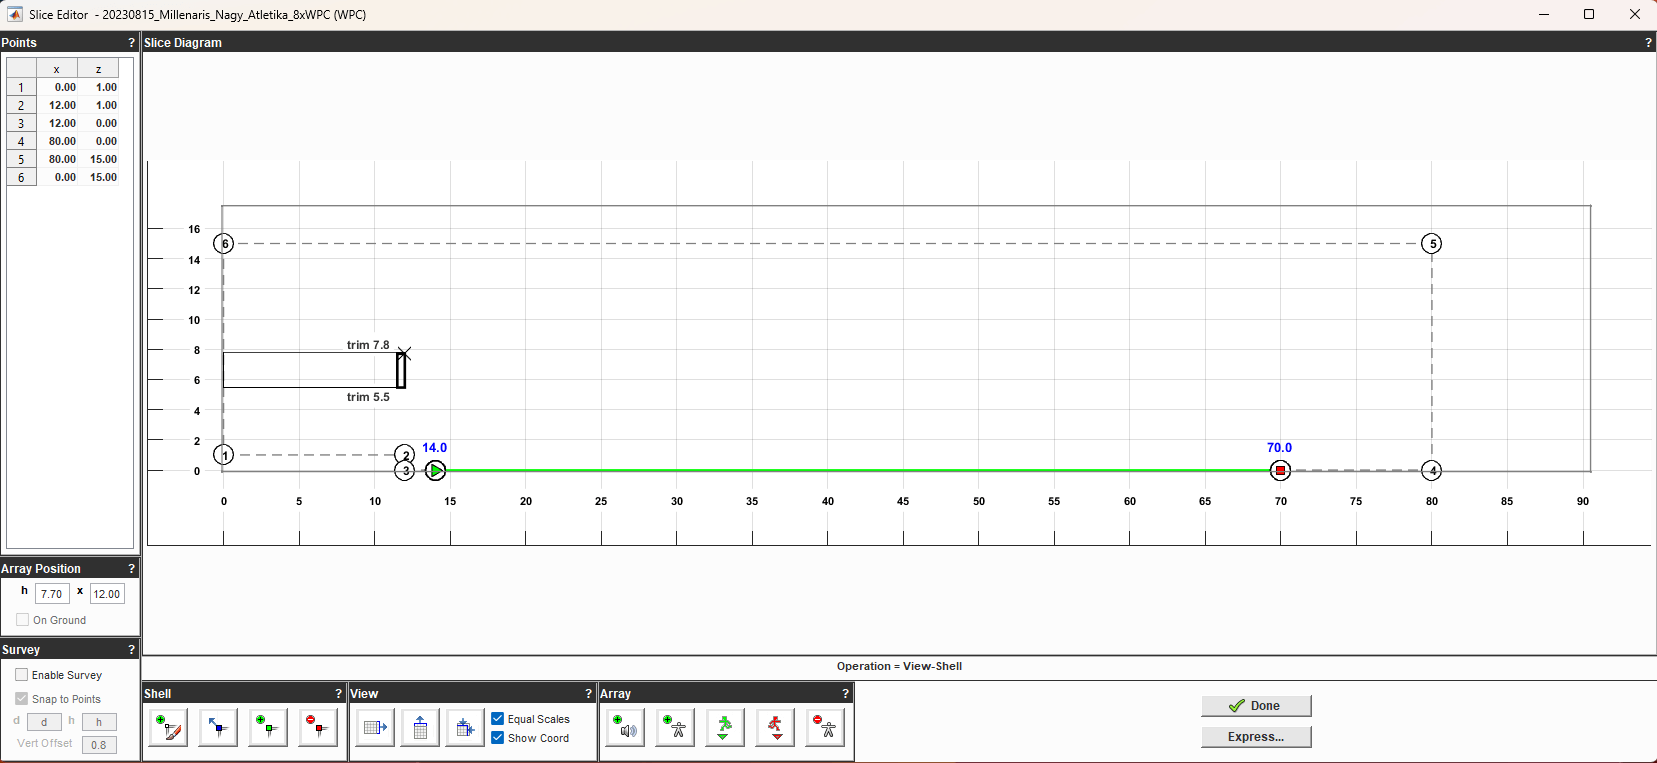
\includegraphics[width=\textwidth, keepaspectratio]{figures/display_wpc_1.png}
	\caption{Display 2.3.4 b1 \textit{``Slice''} kezelőfelülete (WPC)}\label{fig:display_wpc_1}
\end{figure}
%----------------------------------------------------------------------------
A következő lépések a \textit{``Cover''} kezelőfelületen történnek.
Első és legfontosabb beállítás amit el kell végezni, hogy a hallgatóság az esemény során ülni vagy állni fog-e.
Lehetőségünk van a nézőteret különböző részekre is osztani, amennyiben a rendezvény során különböző helyeken
eltérő típusú részeket szeretnénk egyenletesen lefedni. Lehetőség van egyedi magasság beállítására is,
de jelen esetben a közönség egyhangúan állva fogja hallgatni a produkciót, ezért a \textit{``Standing''} opciót választottam.
Az előző lépésben elkészített rajzunkon definiálhatunk a program számára három fő régiót.
\newline Ezek az alábbiak:
%----------------------------------------------------------------------------
\begin{itemize}
	\item \textit{``Non Audience''} - a közönség területén kívül eső terület
	\item \textit{``Audience''} - a közönség területe
	\item \textit{``Hard Avoid''} - a közönség területén kívül eső terület, ahol a hangvisszaverődést szeretnénk minimalizálni
\end{itemize}
%----------------------------------------------------------------------------
Jelen esetben a fő hangrendszernél nem jelöltem meg a \textit{``Hard Avoid''} területet, mivel a teremben az első olyan felület
ami a hangvisszaverődést okozna már olyan távol helyezkedik el a hangrendszertől, hogy a hangvisszaverődés már nem okoz problémát.
A következő lépéseket előkészítve meg kell határoznunk a hangrendszertől egy adott távolságra lévő pontot a teremben,
amit referencia pontként fogunk használni. Ezt a pontot a \textit{``Move Ref''} gombra kattintva tudjuk megadni,
vagy manuálisan beírva az X és Y koordinátákat. Automatikusan a terem közepére van pozícionálva a referencia pont, de
ezt erősen ajánlott mozgatni attól függően mit szeretnénk elérni. Jelen esetben a mix pultot fogjuk a referencia pontnak megadni.
A \textit{``Start''} és \textit{``Stop''} mezőkben meg kell adnunk, hogy a referencia ponttól véve mekkora hangnyomás
deltával szeretnénk dolgozni. Ez azt jelenti, hogy a kezdő, a referencia és a végpont közötti hangnyomás hány dB-el térhet el egymástól.
Ezt az értéket a szoftver az eddig megadott információk alapján automatikusan kiszámolja, de manuálisan is megadhatjuk.
Az automatikus számítás az esetek többségében megfelelő eredményt ad, ezért most is ezt választottam.
A \textit{``Target SPL''} mezőben megadhatjuk a referencia ponton elérni kívánt hangnyomás szintet.
Így a rendszer \textit{``Gain''} struktúrája úgy lesz beállítva, hogy a referencia ponton 0 dBu bemeneti szint mellett elérjük a megadott hangnyomás szintet.
Magas frekvenciák csökkennek ahogy a távolság nő a forrástól, azaz a hangrendszertől.
Ha egyenletes frekvencia választást szeretnénk elérni nagyobb távolságokon, akkor a rendszernek nagyobb energiára lenne szüksége
a magas frekvenciákon, és kifutna a dinamika tartalékból, ezért jobb megoldás, ha a magas frekvenciák fokozatosan csökkennek a távolság növekedésével.
Beállíthatjuk a levegő veszteség kompenzációját, teljesen balra állítva nincs kompenzáció (figyelmen kívül hagyva a levegő abszorpcióját).
Teljesen jobbra állítva a maximális kompenzáció (a rendszernek 17dB headroom-ra van szüksége, hogy egyenes választ kapjunk).
Viszont ezekből az következik, hogyha túlságosan sok a kompenzáció, akkor a rendszernek nem lesz elég dinamika tartaléka, és a hang torzulni fog.
A változások hatását a \textit{``Target Response''} ábrán láthatjuk.
Ahhoz, hogy a számítások pontosak legyenek, elengedhetetlen, hogy pontosan megadjuk a környezeti változókat,
a hőmérsékletet, a páratartalmat és a légnyomást. Ezeket a paramétereket a \textit{``Edit''} gombra kattintva tudjuk megadni.
Jelen esetben mivel a teremben alapból is meleg van, a mérés időpontjában 28 fok, és a rendezvény során a közönség is melegíti a termet,
ezért a hőmérsékletet harminc fokra állítottam.
A páratartalom értéke a méréskor 57\%-os volt, de én 65\%-ra állítottam, mivel a rendezvény során a közönség által kibocsátott
vízgőz miatt a páratartalom nagy valószínűséggel magasabb lesz ennél. A légnyomás értékét pedig a helyi időjárás jelentésből vettem, ami
azon a napon 101800 Pa volt. Ezek beállítása után mivel az adott hangládához a gyári beállítások nagyon jók, ezért nem változtattam rajtuk,
a 14-es érték egyenletes és dinamikus hangvisszaadást biztosít.
%----------------------------------------------------------------------------
\begin{figure}[H]
	\centering
	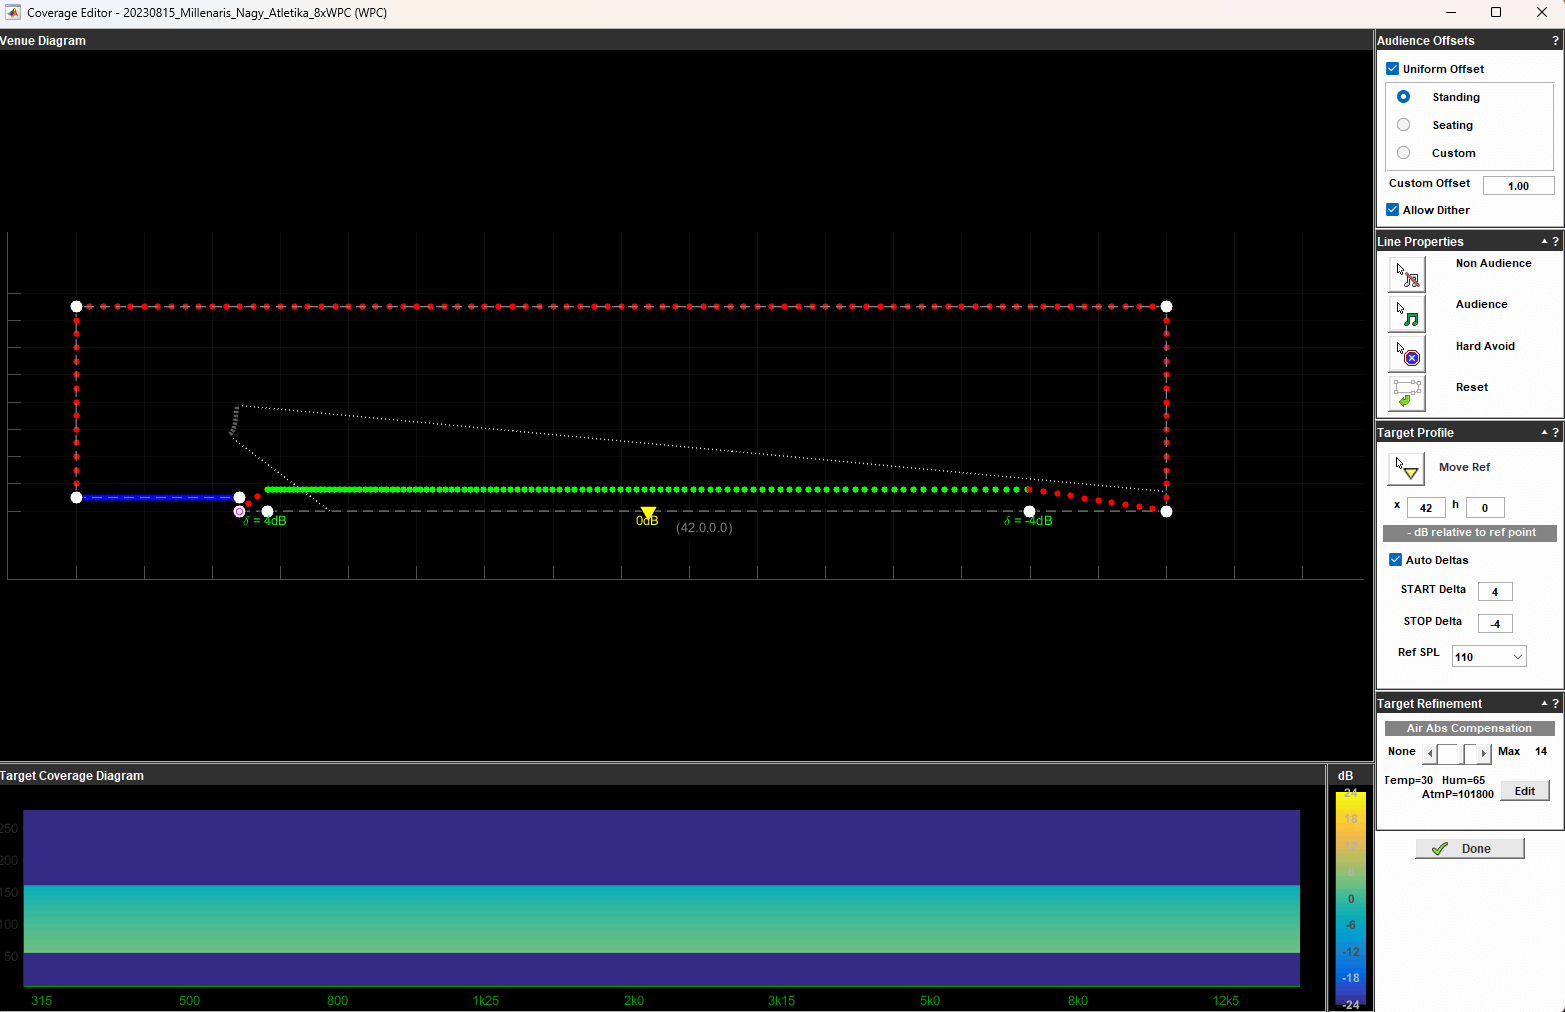
\includegraphics[width=\textwidth, keepaspectratio]{figures/display_wpc_2.png}
	\caption{Display 2.3.4 b1 \textit{``Cover''} kezelőfelülete (WPC)}\label{fig:display_wpc_2}
\end{figure}
%----------------------------------------------------------------------------
Miután a \textit{``Cover''} kezelőfelületen elvégeztük a szükséges beállításokat, a \textit{``Splay''} kezelőfelületen folytatjuk a tervezést.
Az optimalizáció ezen részén a hangrendszert fogjuk a hallgatóság területére irányítani, a fokolási szögek beállításával.
A szoftver által biztosított optimalizációs algoritmus a lehető legjobb lefedettségre törekszik a tervezett területen.
Lehetőség van az optimalizáció súlyozási tényezőinek beállítására, de jelen esetben a gyári beállításokat használtam.
Amennyiben módosítani szeretnénk a súlyozást a \textit{``Target'} és a \textit{``Leakage''} mezőkben tudjuk megadni a súlyozási tényezőket.
A \textit{``Target''} mezőben megadott érték a közönség terület súlyozása,
a \textit{``Leakage''} mezőben megadott érték pedig a közönség területén kívül eső szivárgás súlyozása.
Az \textit{``Alow Polish''} opció engedélyezi a szoftvernek, hogy egy második körben finom hangolja a splay szögeket az első próbálkozás után.
Ezt az opciót előnyös bekapcsolni, mivel a szoftver így pontosabb eredményt tud produkálni, ezért ezt a beállítást mindig használom.
A \textit{``Max Time''} mezőben megadhatjuk, hogy a szoftvernek mennyi idő álljon rendelkezésére az optimalizáció elvégzéséhez.
Mivel a mai modern számítógépek olyan gyorsak, hogy a szoftver általában 1-2 perc alatt elvégzi az optimalizációt, ezért ezt az értéket
nem szoktam módosítani. A \textit{``Max Time''} mezőben megadott érték másodpercben értendő.
%----------------------------------------------------------------------------
\begin{figure}[H]
	\centering
	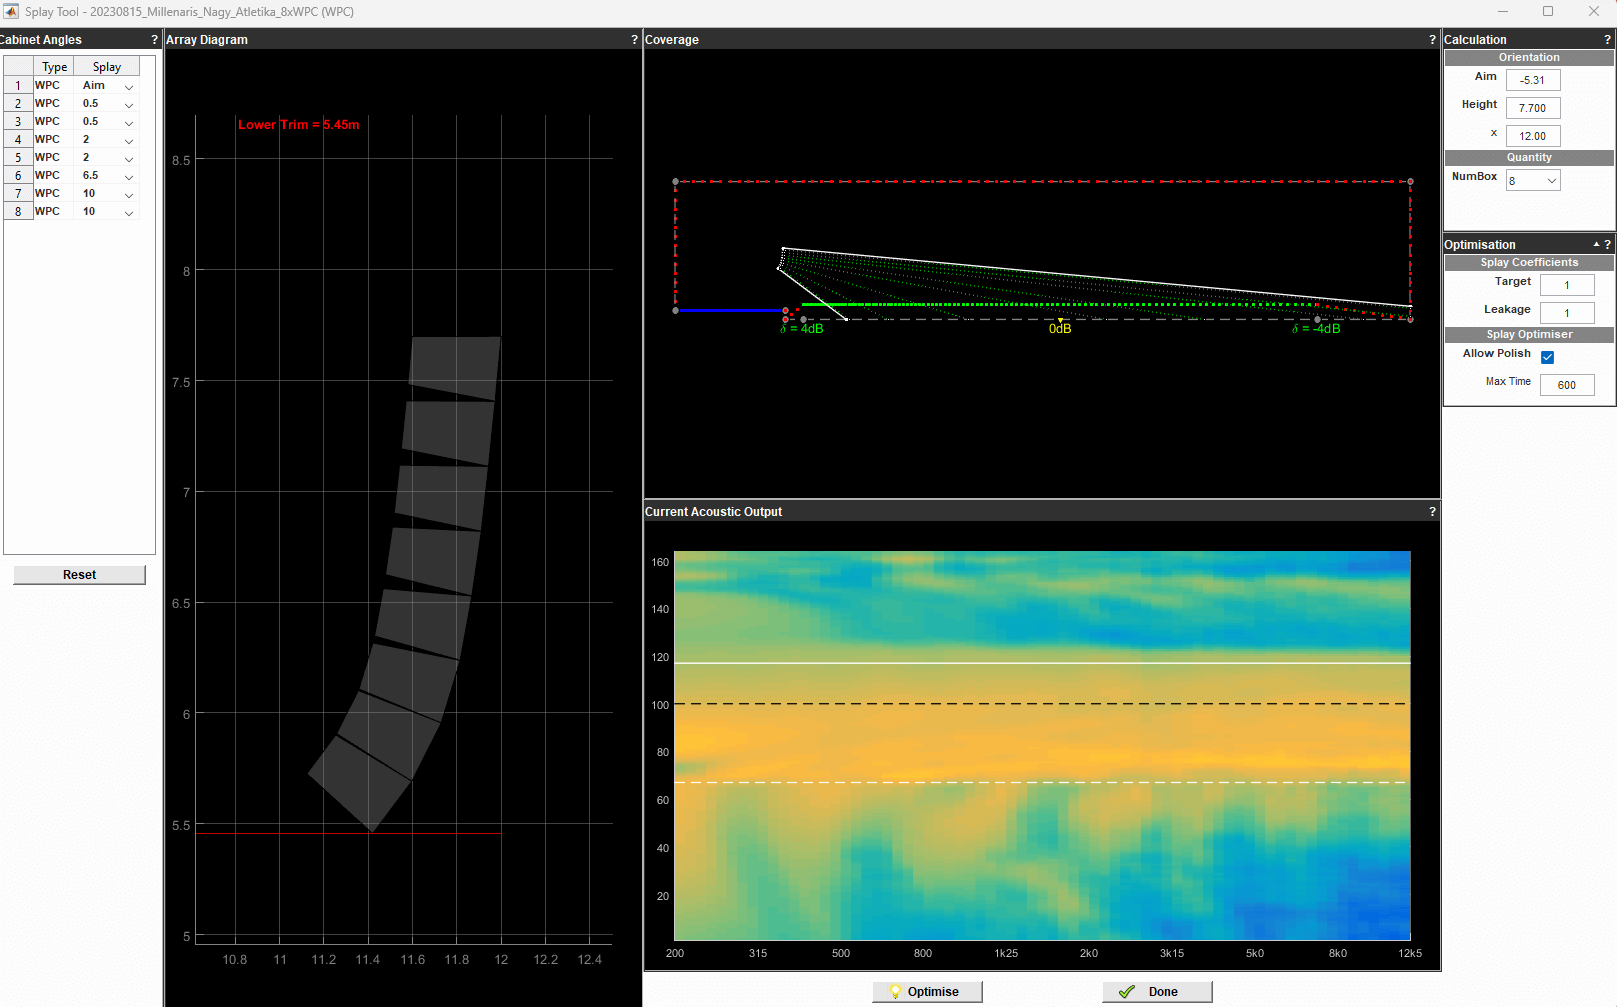
\includegraphics[width=\textwidth, keepaspectratio]{figures/display_wpc_3.png}
	\caption{Display 2.3.4 b1 \textit{``Splay''} kezelőfelülete (WPC)}\label{fig:display_wpc_3}
\end{figure}
%----------------------------------------------------------------------------
A következő lépés a \textit{``Rig''} kezelőfelületen történik. Ez a felület elsősorban az eddig elkészített
rendszerünket fogja megjeleníteni térben. Elsődleges beállítási paraméter ezen a panelen, hogy egy vagy két pontos
rögzítést szeretnénk-e használni. Jelen esetben egy pontos  rögzítést fogunk használni. Amennyiben valamilyen okból
szeretnénk változtatni a rendszer fizikai elhelyezkedésén, még megtehetjük, de ez a lépés ezen a ponton már nem ajánlott.
Bármely kis apró változtatás kardinálisan más végeredményhez vezethet. A tervezési folyamatot újra kell kezdeni, ellenkező esetben
a szoftver nem fogja tudni a megfelelő eredményt produkálni, és a rendszerünk nem úgy fog viselkedni a valóságban, ahogy azt mi szeretnénk.
A hangrendszer függesztéséhez és összeszereléséhez az összes információ megtalálható itt. Gondolva itt a riggvas fokolási helyére,
a ládák közti szögekre, a rendszer legfelső és legalsó pontjára.
Ezeken az információkon kívül még a rendszer súlyát és súlypontját is megkapjuk.
Esetünkben a teljes súly 289 kilogramm, amit a csarnok tartószerkezete biztonságosan elbír, valamint az egy tonnás emelőkapacitású
láncos emelők is képesek biztonságosan emelni. A súlypont a rendszer relatíve közepén helyezkedik el, ami stabil függesztést tesz lehetővé.
Ezek után a rendszert az említett paraméterek alapján össze építjük, figyelve az összes program által megadott információra.
%----------------------------------------------------------------------------
\begin{figure}[H]
	\centering
	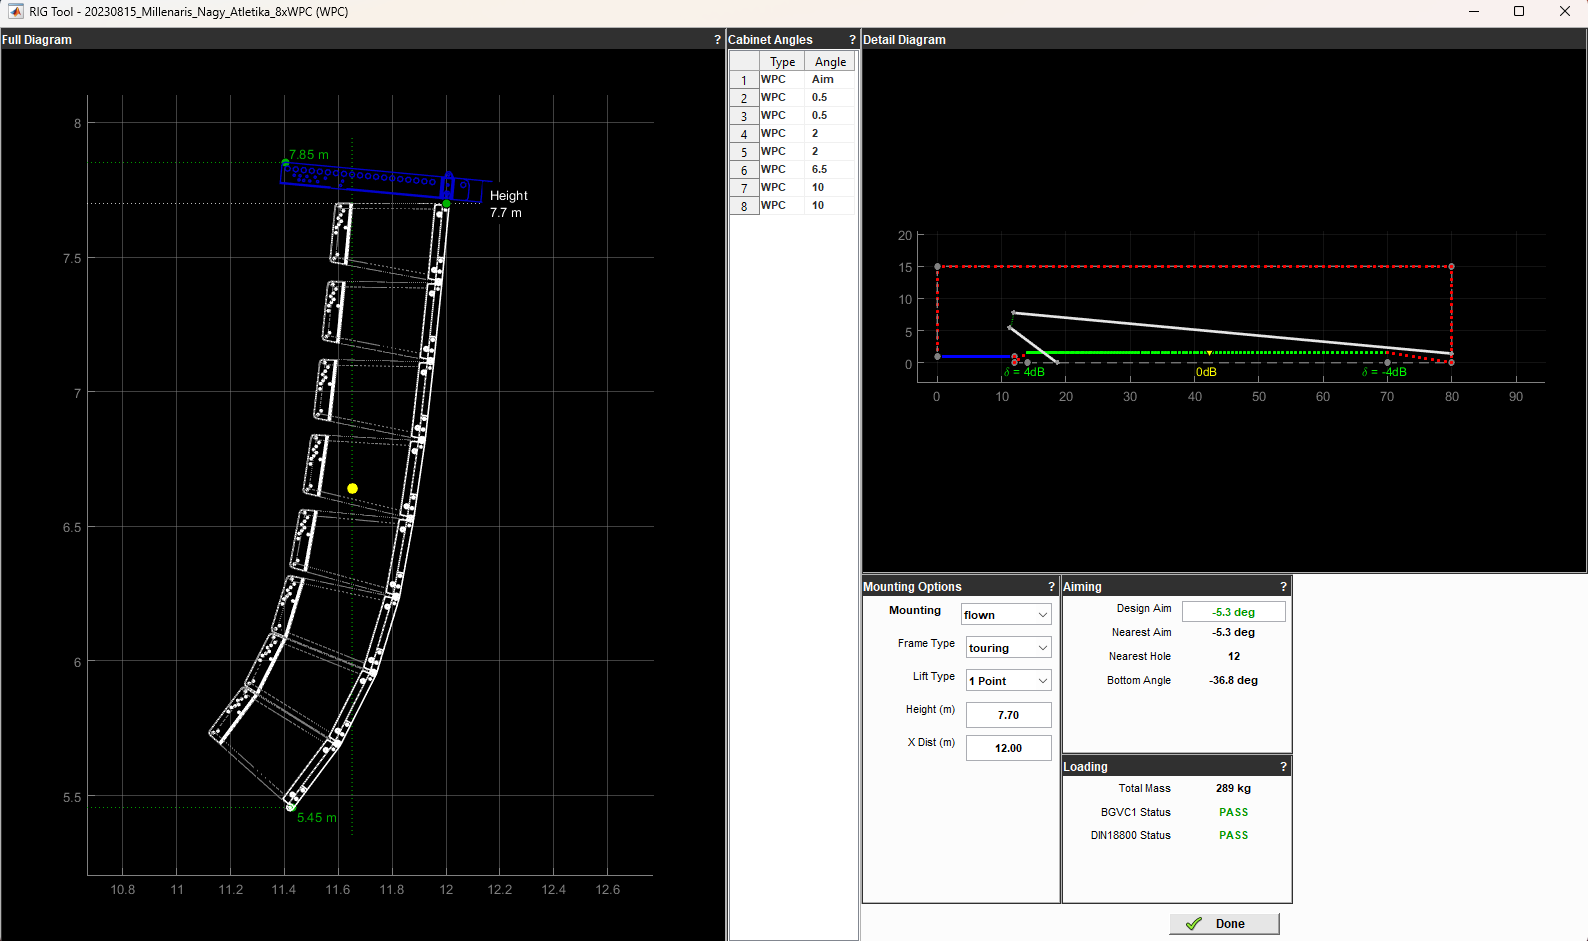
\includegraphics[width=\textwidth, keepaspectratio]{figures/display_wpc_4.png}
	\caption{Display 2.3.4 b1 \textit{``Rig''} kezelőfelülete (WPC)}\label{fig:display_wpc_4}
\end{figure}
%----------------------------------------------------------------------------
Az utolsó lépés mielőtt ki tudnánk menteni a tervezett rendszert, az a \textit{``EQ''} kezelőfelületen történik.
Ha a \textit{``Cover''} kezelőfelületen már megadtuk a környezeti változókat, akkor ezt már nem kell újra megtennünk,
mivel a szoftver automatikusan átveszi az ott megadott értékeket. Beállíthatjuk az alsó és felső határfrekvenciákat, de mivel
a program a kiválasztott hangrendszerhez tartozó gyári beállításokat automatikusan betölti, ezért ezeket az értékeket sem kell módosítani.
Amit viszont érdemes és erősen ajánlott módosítani, az a \textit{``Freq Res''} és a \textit{``Space Res''} értékek. Az előbbi a
frekvencia felbontást, az utóbbi pedig a térbeli felbontást jelenti. Ezek az értékek határozzák meg, hogy a szoftver milyen 
felbontásban végezze el a számításokat. Minél kisebb értéket adunk meg, annál pontosabb eredményt fogunk kapni, viszont a számítások
hosszabb ideig fognak tartani. A \textit{``Freq Res''} értékét 1-re, a \textit{``Space Res''} értékét pedig szintén 1-re állítottam, mivel
ez az elérhető legnagyobb felbontás, és a számításokat is a lehető legpontosabban szeretném elvégezni. A gyári érték mindegyiknél a kettő.
Minél pontosabbak a számítások, annál jobban fog viselkedni a rendszer a valóságban és egyenletesebb hangvisszaadást fog produkálni.
Ha már a kiegyensúlyozott hangvisszaadásnál tartunk, akkor a \textit{``Resolution''} panelen meg kell adnunk, hogy milyen
konfigurációban szeretnénk használni a rendszert. A WPC szériás hangládákat tudjuk akár egyesével hajtani, azaz egy láda egy végfok csatorna
párral (mivel Bi-Amp hangládáról beszélünk). De a gyártó lehetőséget biztosít arra is, hogy a ládákat párosával vagy hármasával is hajtsuk.
Ennek költséghatékonysági és rugalmassági előnyei vannak, viszont a hangvisszaadás kevésbé lesz egyenletes. Jelen esetben 
az arany középutat választottam, és párosával fogom hajtani a ládákat. Így a rendszer összesen 3 darab iK42 végfokot fog igényelni, ami 
12 darab végfokcsatornát jelent. A WPC rendszer csak iK42 végfokkal hajtható, a 8 csatornás iK81 végfokkal nem kompatibilis.
Lehetőség van az optimalizációs algoritmus befolyásolására is, a három előbbiekben már definiált súlyozási tényezők segítségével.
A fő hangsúlyt a \textit{``Target''} súlyozásra helyeztem, mivel a közönség területén szeretném a lehető legjobb hangvisszaadást elérni,
ezért 60\%-os súlyozást adtam neki.
A \textit{``Hard Avoid''} és a \textit{``Leakage''} súlyozását 20\%-ra állítottam.
Továbbá mindhárom résznek megadhatjuk mekkora hangnyomás értéket szeretnénk elérni a tervezett területen. Ezeket az értékeket
nem szükséges módosítani, mivel a gyári értékek megfelelőek, de ha mégis szeretnénk, akkor megtehetjük.
A paraméterezés után az optimalizáció után megkapjuk a teljes rendszer EQ beállítását és vizuális ábrázolást kapunk 
a referencia értéktől való eltérésekről.
%----------------------------------------------------------------------------
\begin{figure}[H]
	\centering
	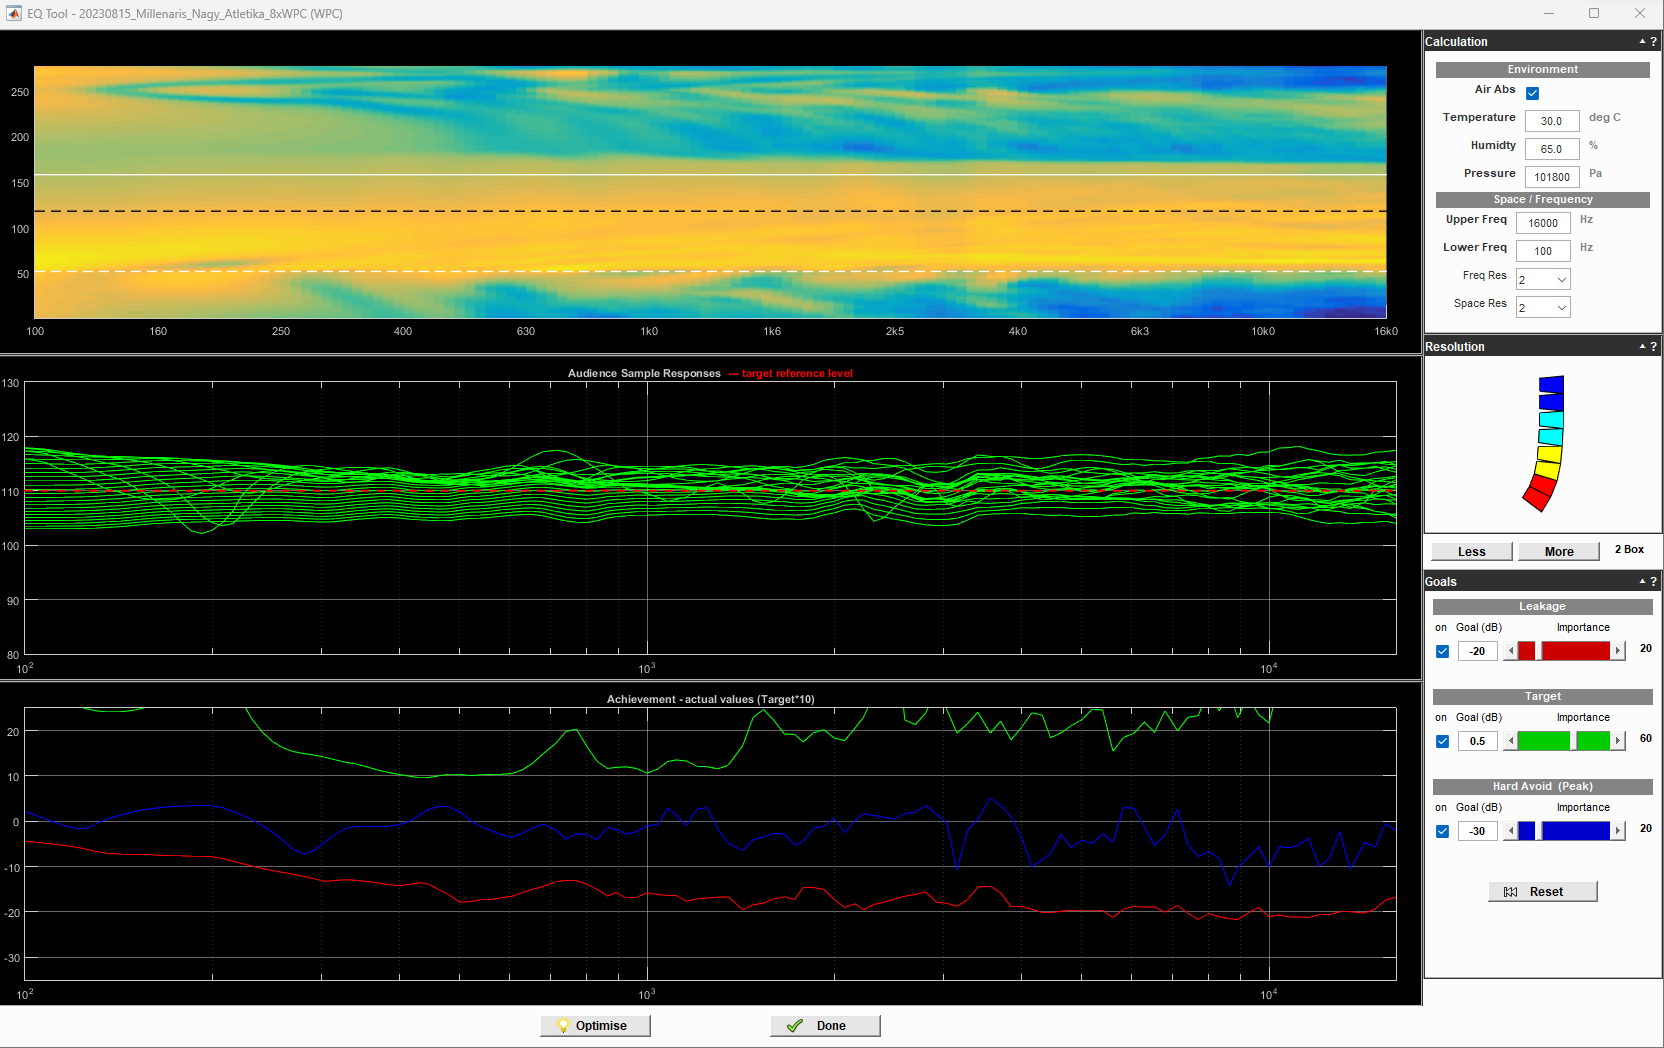
\includegraphics[width=\textwidth, keepaspectratio]{figures/display_wpc_5.png}
	\caption{Display 2.3.4 b1 \textit{``EQ''} kezelőfelülete (WPC)}\label{fig:display_wpc_5}
\end{figure}
%----------------------------------------------------------------------------
%Amennyiben szeretnénk megtekinteni a tervezett rendszer teljesítményét amit a program számított ki, 
%akkor az \textit{``SPL''} kezelőfelületen, az \textit{``Index Plot''}-on a bal egeret nyomva tartva
%tudunk virtuálisan mozogni a teremben, és megtekinthetjük a számított hangnyomás és frekvencia eloszlás értékeket.
%Ha mindent rendben találunk és nincsenek kivetnivalóink a tervezett rendszerrel kapcsolatban, akkor
%sikeresen megterveztük a hangrendszert, és elmenthetjük a projektet.
%A mentés során egy MAT kiterjesztésű fájlt fogunk kapni, segítségével később bármikor újra megnyithatjuk a projektet,
%ha ugyan azon a helyszínen dolgozunk, gyorsabban és egyszerűbben tudjuk a rendszert újra tervezni, a szükséges
%módosításokat elvégezni.
%----------------------------------------------------------------------------
%\begin{figure}[H]
%	\centering
%	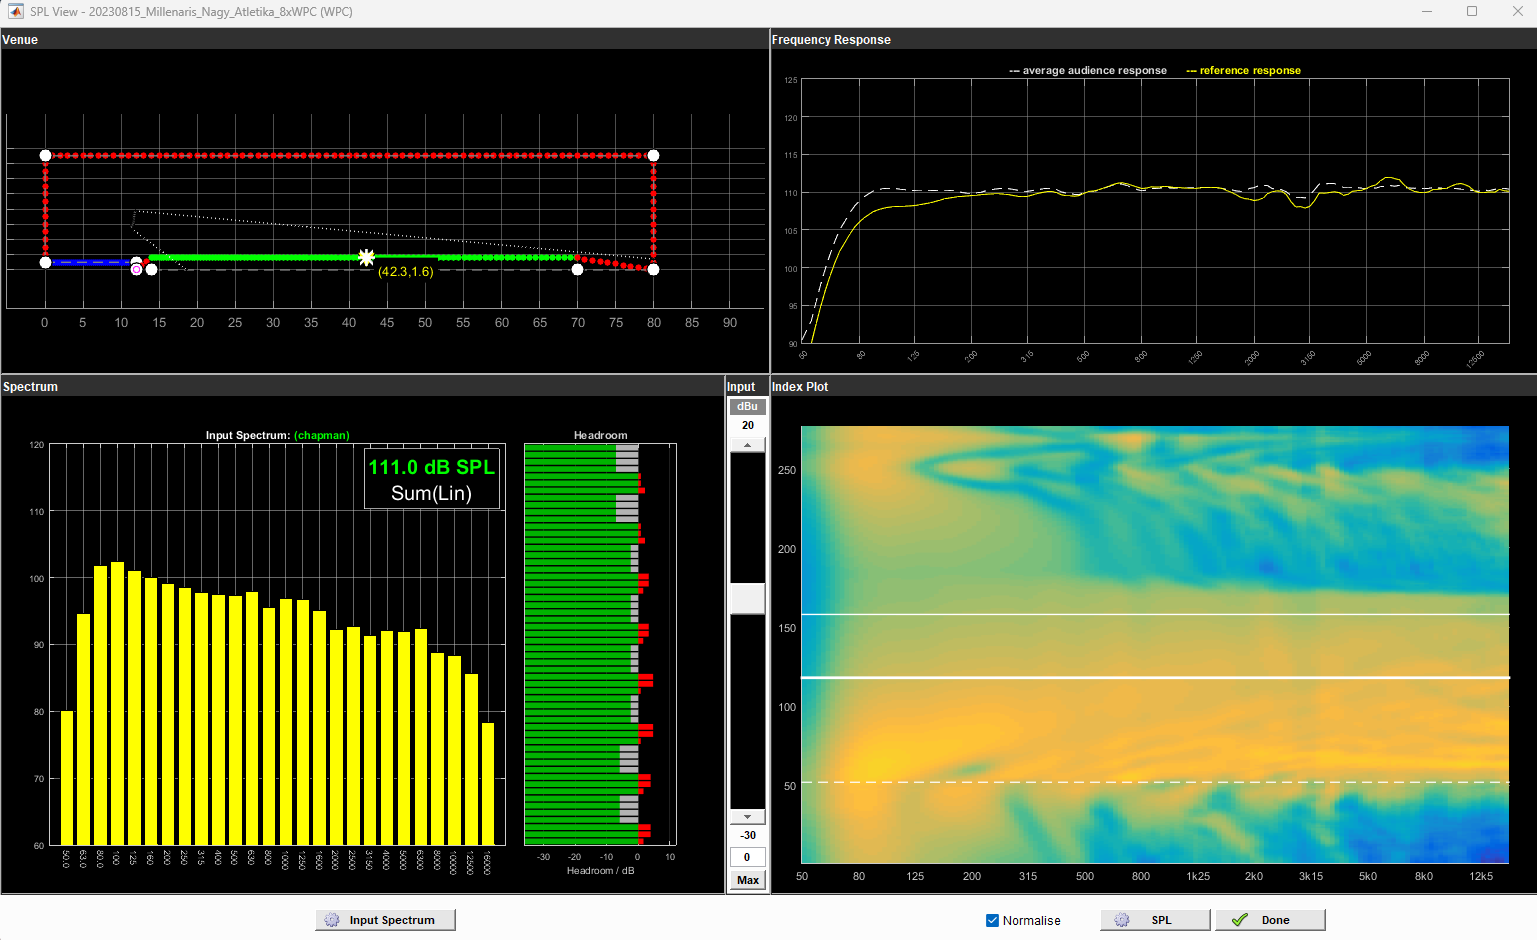
\includegraphics[width=\textwidth, keepaspectratio]{figures/display_wpc_6.png}
%	\caption{Display 2.3.4 b1 \textit{``SPL''}kezelőfelülete (WPC)}\label{fig:display_wpc_6}
%\end{figure}
%----------------------------------------------------------------------------
Az utolsó dolgunk ebben a programban mielőtt tovább lépünk, hogy exportáljuk a tervezett rendszert.
Az exportálás során egy D2P kiterjesztésű fájlt fogunk kapni, amit a VU-NET szoftver fog tud majd importálni a későbbiekben.
%----------------------------------------------------------------------------
\begin{figure}[H]
	\centering
	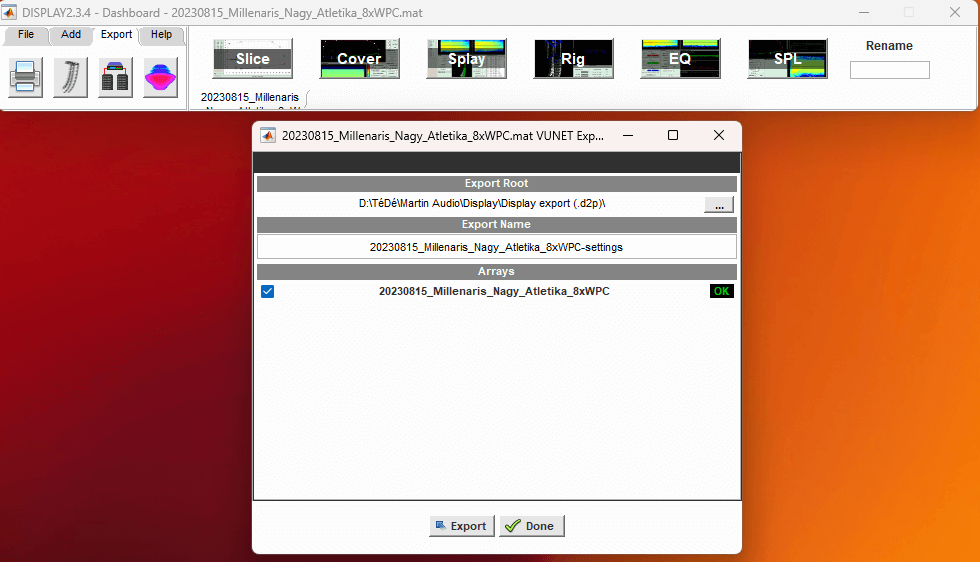
\includegraphics[width=\textwidth, keepaspectratio]{figures/display_wpc_7.png}
	\caption{Display 2.3.4 b1 exportáló kezelőfelülete (WPC)}\label{fig:display_wpc_7}
\end{figure}
%----------------------------------------------------------------------------
A fő hangrendszer megtervezése után a következő részegység aminek a tervét el kell készíteni, az a Delay hangrendszer.
A Delay hangrendszer a fő hangrendszerrel együtt fog működni, és a közönségtér hátsó-közép részétől kezdve fogja kiegészíteni azt.
Erre azért van szükség, mert a csarnokban a közönség ezen része olyan távolságra helyezkedik el, hogy
a WPC rendszer már nem tudja a megfelelő hangnyomás szintet egyenletesen biztosítani.
Ezt a feladatot a Wavefront Precision sorozatból a WPM típusú hangládák fogják ellátni, oldalanként 6-6 darab LineArray modullal.
Ez a láda egy két utas passzív hangrendszer, 2 darab 6.5"-os mély hangszóróval (LF) és 3 darab 1.4"-es magas hangszóróval (HF). 
Maximásan 130 dB hangnyomás szintet tud biztosítani, nagy előnye ennek a fajta rendszernek a súly-teljesítmény aránya, mivel egy
darab láda mindössze 14 kilogramm. \cite{WPMUSERGUIDE}
%----------------------------------------------------------------------------
\begin{figure}[H]
	\centering
	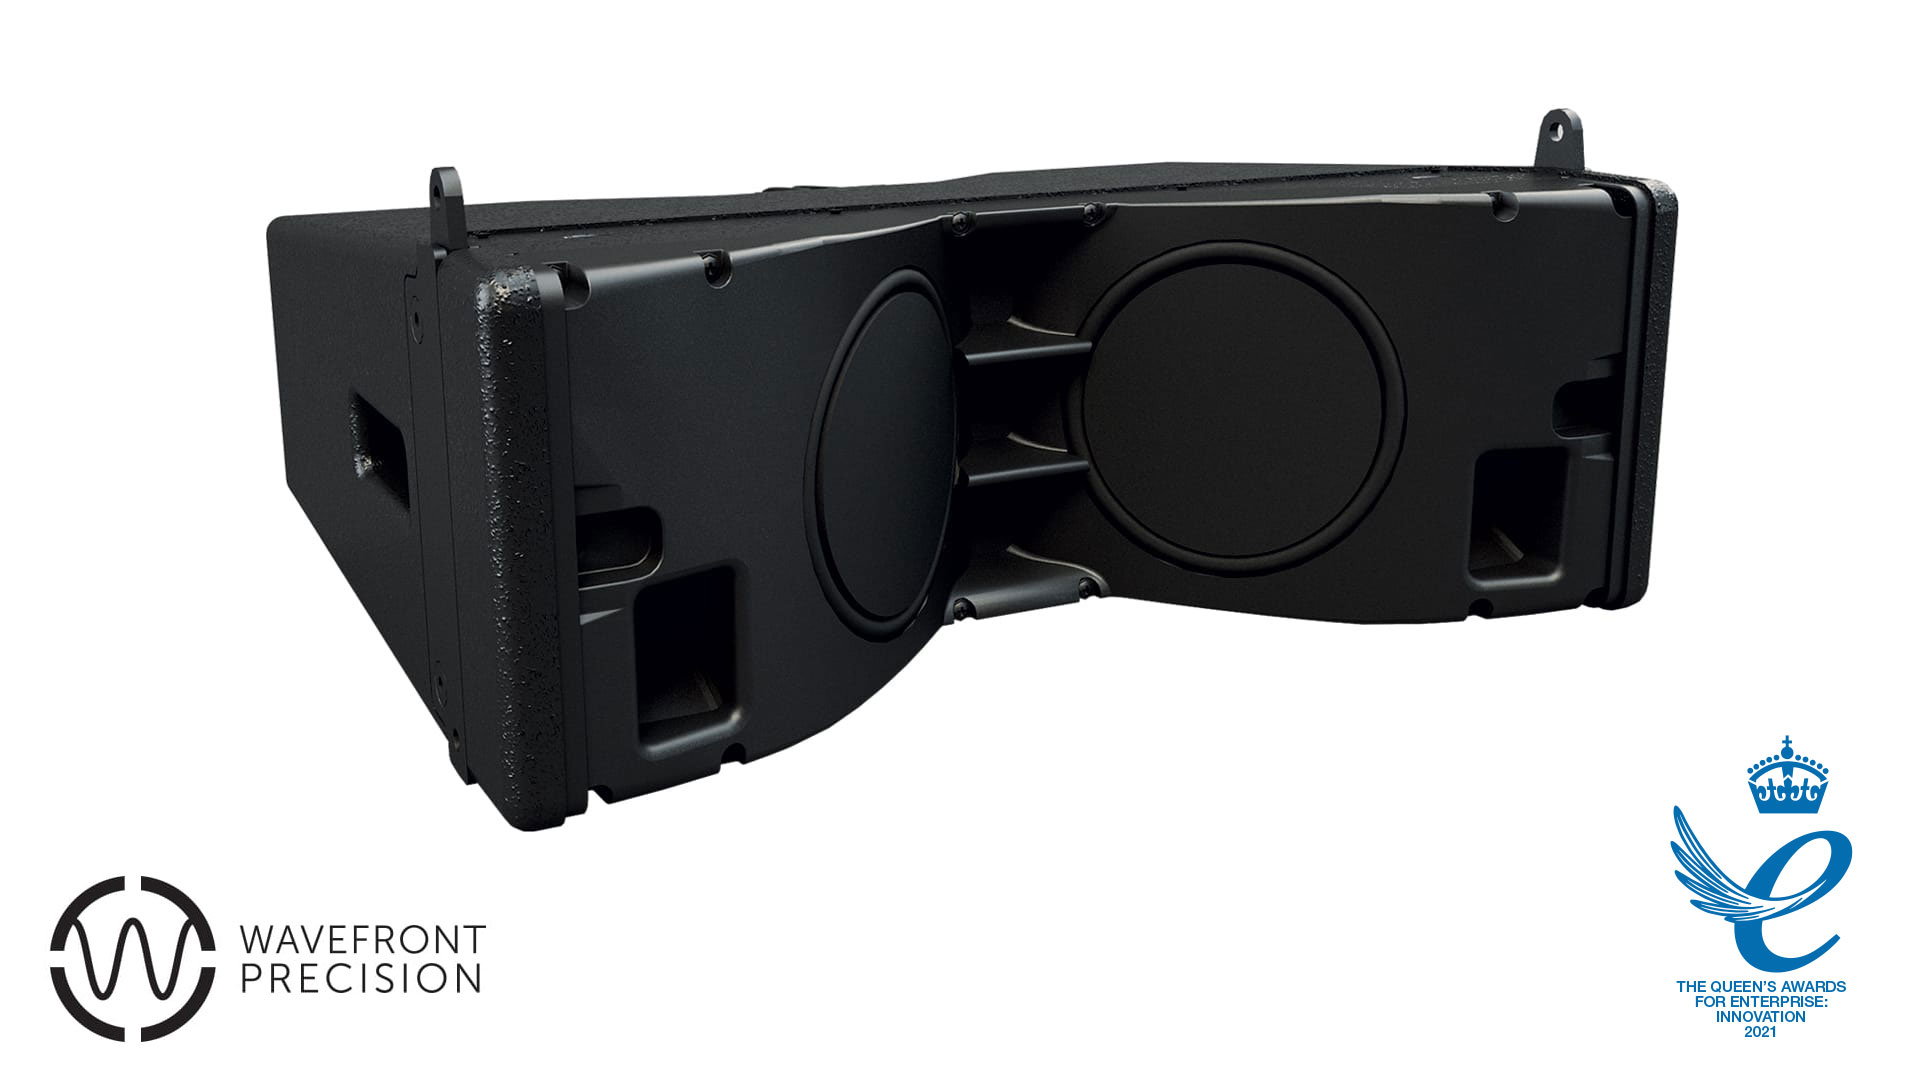
\includegraphics[width=80mm, keepaspectratio]{figures/wpm_front_view.jpg}
	\caption{Martin Audio WPM LineArray modul}\label{fig:wpm}
\end{figure}
%----------------------------------------------------------------------------
A tervezési fázisok nagy része megegyezik az előbbi rendszer tervezésével, ezért ezeket a részeket nem ismétlem meg.
A hangsúlyt a eltérésekre helyezem, és azokat fogom részletezni.
A fő különbség a \textit{``Cover''} kezelőfelületen történik, ahol a \textit{``Hard Avoid''} területet kell megjelölni.
Ezen a rajzon már radikálisan szükség van erre a funkcióra, mivel a közönség területén kívül eső területen beton nagy felületek találhatóak,
amelyek jelentős hangvisszaverődést okoznának. 
%----------------------------------------------------------------------------
%\begin{figure}[H]
%	\centering
%	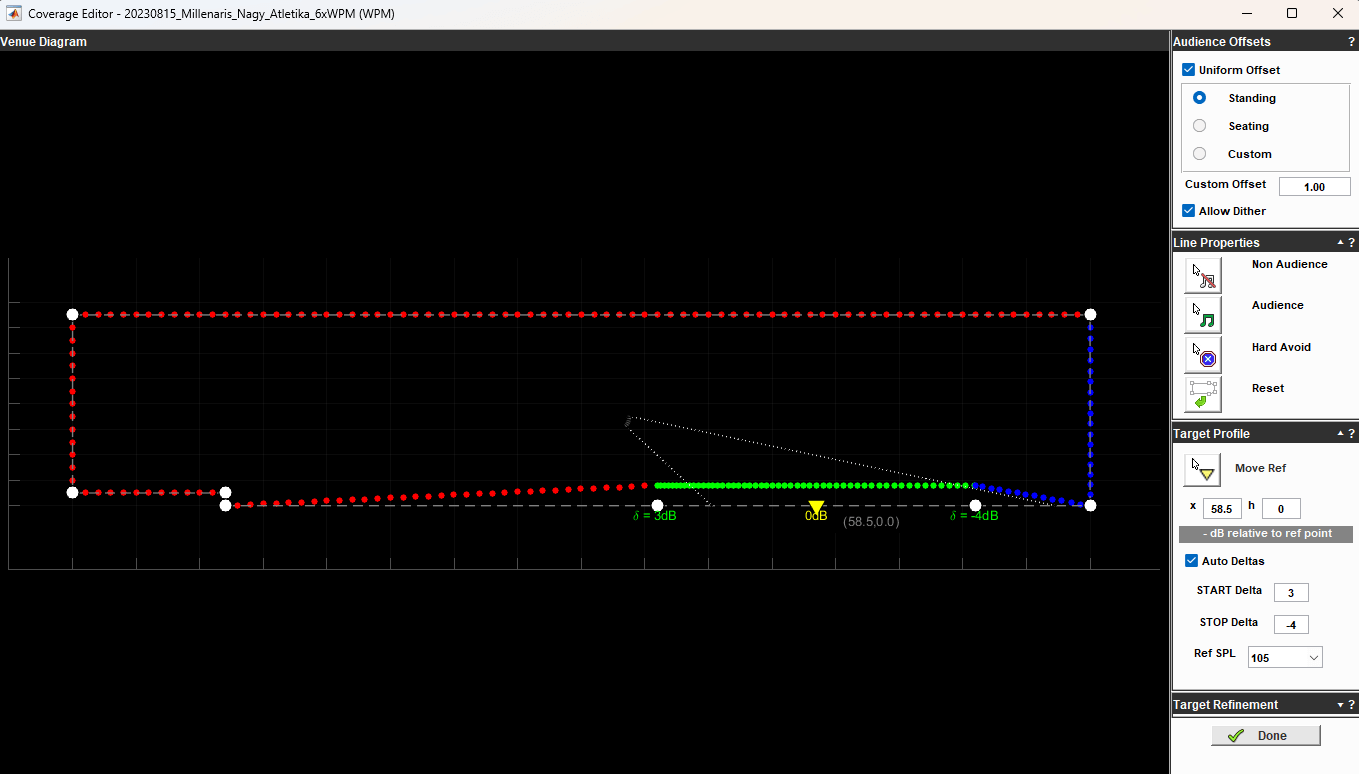
\includegraphics[width=\textwidth, keepaspectratio]{figures/display_wpm_1.png}
%	\caption{Display 2.3.4 b1 \textit{``Cover''} kezelőfelülete (WPM)}\label{fig:display_wpm_1}
%\end{figure}
%----------------------------------------------------------------------------
Ebből kifolyólag, szépen látható, hogy a program pontosan úgy optimalizálja a rendszert, hogy a \textit{``Hard Avoid''} területre, minél kevesebb
hangnyomás jusson.
Már a kék színnel jelölt terület első pár méterén radikálisan csökken a hangnyomás, és a rendszer a lehető legkevesebb energiát fordítja erre a területre.
A gyártó a WMP rendszert végfog csatornák szempontjából úgy tervezte, hogy a költség és a rugalmasság szempontjából akár négyesével is hajthatóak legyenek.
Ez persze nem jár kompromisszumok nélkül, a hangvisszaadás egyenletesebb lenne, ha egyesével hajtanánk a ládákat, de a jelenlegi rendszerben
hármasával fogom hajtani a ládákat, mivel ez a legköltséghatékonyabb megoldás, és végeredményben így is kielégítő hangvisszaadást fog produkálni mint 
kiegészítő egység.
%----------------------------------------------------------------------------
\begin{figure}[H]
	\centering
	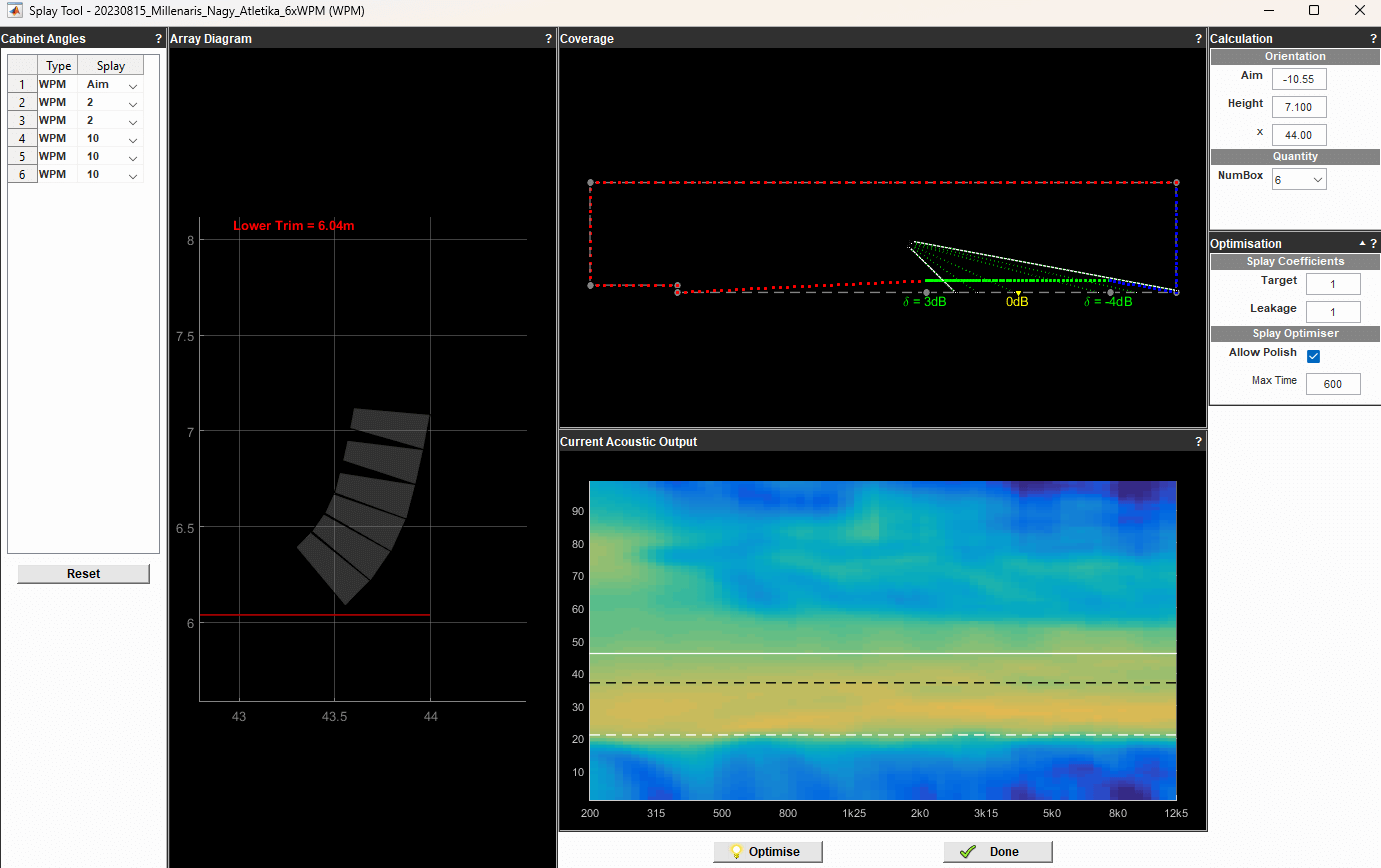
\includegraphics[width=\textwidth, keepaspectratio]{figures/display_wpm_2.png}
	\caption{Display 2.3.4 b1 \textit{``Splay''} kezelőfelülete (WPM)}\label{fig:display_wpm_2}
\end{figure}
%----------------------------------------------------------------------------
Az előbbiekben már tárgyalt exportáló felületen az összes többi optimalizációs lépést követően
mentjük az elkészített tervet a WPC rendszerhez hasonlóan.
%----------------------------------------------------------------------------
\subsubsection{Martin Audio VU-NET rendszer szoftver \cite{VUNETUSERGUIDE}}
%----------------------------------------------------------------------------
Miután már rendelkezünk az összes számunkra szükséges tervezett rendszerrel a rendezvényhez, a következő lépések a VU-NET szoftverben történnek.
A VU-NET szoftver egy olyan alkalmazás, amely lehetővé teszi a Martin Audio hangrendszerek teljes körű vezérlését és monitorozását.
Jelen esetben az iK42 és iK81 típusú végfokokat fogjuk tudni kezelni. 

%----------------------------------------------------------------------------
\subsubsection{Mélyláda rendszer}
%----------------------------------------------------------------------------
A mélyláda hangja hosszabb hullámhosszú, mint a többi komponensé, ezért az
optimális helymeghatározásuk és elhelyezésük kulcsfontosságú a megfelelő
hangzás érdekében. 
A rendszerben a Martin Audio SX218 típusú mélyládáit fogjuk használni.
Ezek a ládák dupla 18"-os mély hangszórókkal vannak felszerelve, 2000W AES és 8000W csúcsteljesítményre képesek, és
maximálisan 144 dB hangnyomás szintet tudnak biztosítani. \cite{SXSUBWOOFERUSERGUIDE}
%----------------------------------------------------------------------------
\begin{figure}[H]
	\centering
	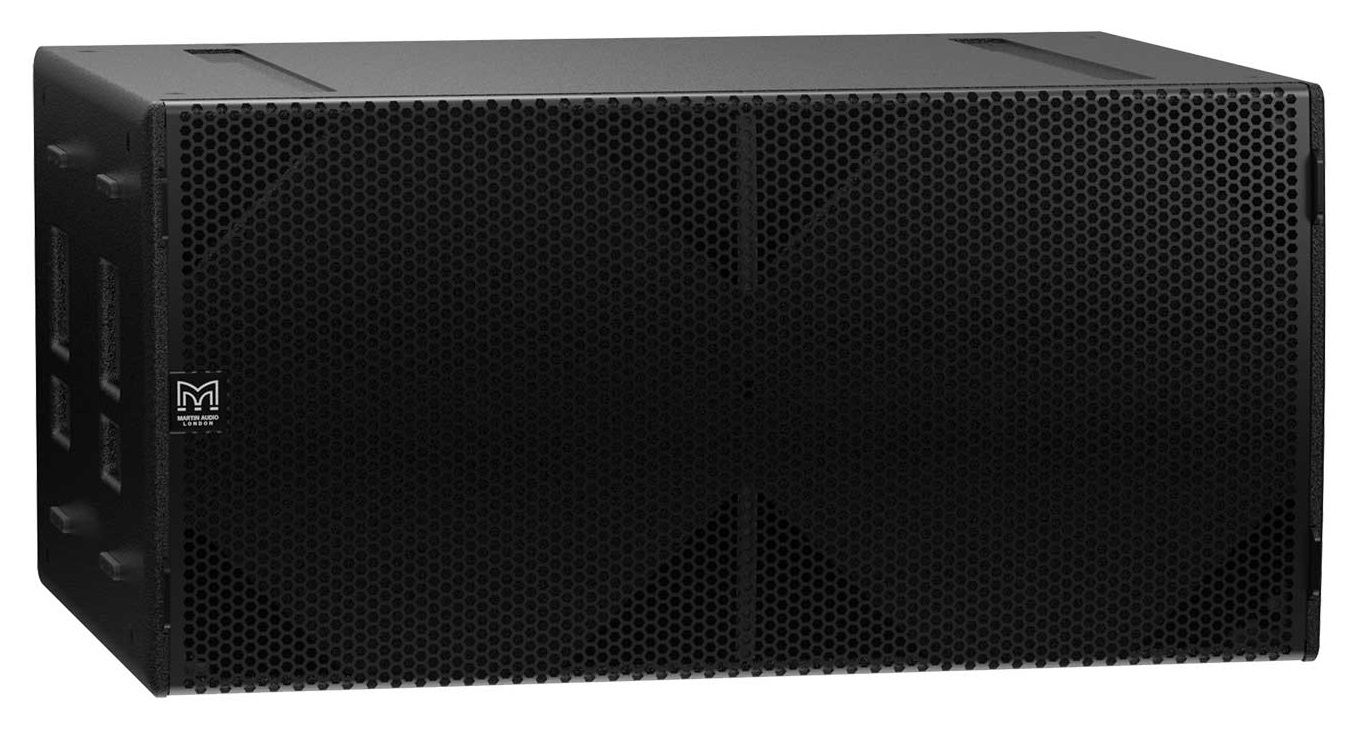
\includegraphics[width=80mm, keepaspectratio]{figures/sx218_front_view.jpg}
	\caption{Martin Audio SX218 mélyláda}\label{fig:sx218}
\end{figure}
%----------------------------------------------------------------------------
A \textit{``SUB''} tervezést egy általam készített Excel kalkulátor
segítségével végzem el. Ez a táblázat egyesíti a Martin Audio és Merlin van Veen által
készített kalkulátorokat (S.A.D), valamint kiegészítésre került további modulokkal és funkciókkal. \cite{MERLINVANVEEN} \cite{MARTINSUBCALCULATOR}
A egy EndFire konfigurációs mélyláda elrendezést terveztem. 
(Egy EndFire Pack = két láda egymás előtt adott távolságra és késleltetési értékkel) 
A táblázatba megadhatjuk, hogy éppen helyileg hol
van a rendezvény, és egy időjárás API segítségével megkapjuk az adott napra/napokra a
teljes időjárás előrejelzést. Majd ezekből egy adott időintervallumra átlagolva
megkapjuk az optimális értékeket a tervezéshez. 
A program kiszámolja, hogy milyen távolságra kell a ládákat helyezni egymástól előrefelé,
valamint mekkora \textit{``delay''} értéket kell alkalmazni. 
Majd az egyes EndFire Pack-ok egymáshoz képesti távolságot oldalirányban és azok
közötti delay értéket is megkapjuk. A \textit{``SUB array''}-t 63 Hz-re optimalizáltam, mivel
ez az a frekvenciatartomány, ahol a mélyláda rendszer a legtöbb energiát tudja leadni.
%----------------------------------------------------------------------------
\subsection{Allen \& Heath digitális keverőrendszer}
%----------------------------------------------------------------------------
A jelenlegi rendszer két keverőpultot fog tartalmazni, egyet a fő hangrendszerhez, és egyet a monitor rendszerhez.
Mindkét keverőpult Allen \& Heath SQ-6 típusú digitális keverőpult lesz.
A pultok 96 kHz-es mintavételezési frekvenciával operálnak és 48 csatornát képesek maximálisan kezelni, melyek közül 
24 csatornával rendelkezik fizikailag beépített mikrofon előerősítővel. A konzolokon található 16 programozható gomb,
25 fader melyek 6 rétegben helyezkednek el és a felhasználó személyre szabhatja őket a saját igényei szerint. 
Emellett 12 sztereó mix áll a rendelkezésünkre, melyeket szintén a felhasználó konfigurálhat saját igényei szerint.
A sztereóm mixek testreszabásával tudunk csoportokat is létrehozni.
A konzolokon 8 sztereó effekt motort is megtalálunk, ezekbe a virtuális effekt processzorokba a pultokon található ingyenes és fizetős 
pluginokat tudjuk betölteni. (amennyiben megvásároltuk a fizetős csomagokat, jelen rendszerben ezek nincsenek megvásárolva)
További előnye a platformnak, hogy egy 32x32 csatornás USB audio interfésszel rendelkezik, így a számítógéphez csatlakoztatva
egy nagy felbontású hangkártyaként is használhatjuk. \cite{AHSQ}
%----------------------------------------------------------------------------
\begin{figure}[H]
	\centering
	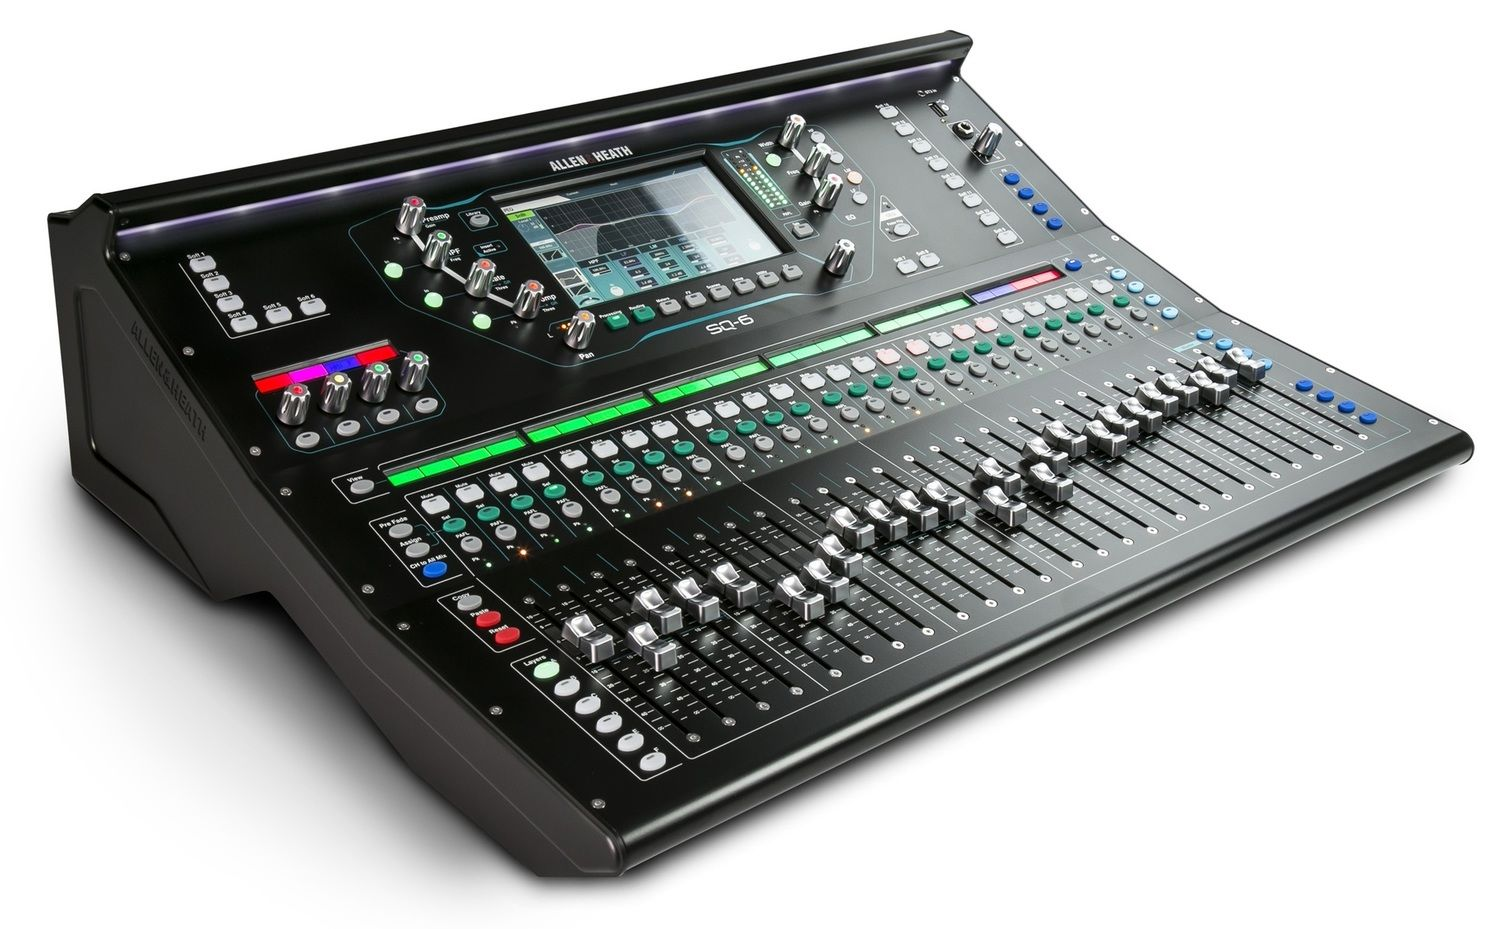
\includegraphics[width=80mm, keepaspectratio]{figures/sq6.jpg}
	\caption{Allen \& Heath SQ-6 digitális keverőpult}\label{fig:sq6}
\end{figure}
%----------------------------------------------------------------------------
\subsection{Shure ULXD digitális vezeték nélküli mikrofonrendszer}
%----------------------------------------------------------------------------
Manapság egy rendezvényen elengedhetetlen a vezeték nélküli mikrofonok használata.
%----------------------------------------------------------------------------
\subsection{Dante audio szerver}
%----------------------------------------------------------------------------
Ez a kiegészítő szerver egység lehetővé teszi bármilyen alacsony késleltetéssel dolgozó VST3 plugin használatát a rendszerben elő környezetben.
Olyan komplex funkcionalitásokat is elérhetünk, amelyek a keverőpulton csak limitáltan, vagy egyáltalán nem elérhetőek.
Gondolva itt a dinamikus EQ használatára, különböző kompressziós technikákra (például Opto, Multiband), 
A legnagyobb előnye ennek a fajta megoldásnak, hogy költségek szempontjából egy magasabb kategóriás keverőpult rendszer sokkal drágább lenne,
valamint nem vagyunk korlátozva a keverőpult által biztosított funkcionalitásokkal, bármikor tudunk igényeink szerint újabb és újabb pluginokat
telepíteni a rendszerbe, amíg a számítógép hardveres erőforrásai ezt lehetővé teszik.
Az általam épített szerver egy AMD Ryzen 7950X processzorral és 32 GB DDR5 memóriával, és a Focusrite RedNet PCIe kártya veszi fel a harcot a
komplex hangfeldolgozási feladatokkal. Ezekre a hardverekre azért esett a választás, mert mivel a Dante kártya 128 csatornát tud kezelni, 
(az épített rendszer 64 csatornás, de a bővítés lehetősége fent áll) erős számítási kapacitásra van szükség, hogy a rendszer a beállított
késleltetési értékek mellett is képes legyen késés nélkül a csatornák feldolgozására. Amennyiben nem sikerül a jelet a beállított időn belül
produkálni, furcsa zavaró pattogó hangokat hallhatunk, vagy rosszabb esetben hangkimaradás is előfordulhat. Ezért fontos a megfelelő hardveres
erőforrások biztosítása, és a pontos beállítások elvégzése.
A példában szereplő rendszer kifogástalanul képes elvégezni a feladatát, és a beállított 1 ms-os késleltetési értéket is képes folyamatosan tartani.
%----------------------------------------------------------------------------
% !!! Képernyőfotó a szerverről !!!
%----------------------------------------------------------------------------
\subsection{Dante hálózat kialakítása és optimalizálása}
%----------------------------------------------------------------------------
\subsubsection{Dante Controller: Hálózati mátrix}
%----------------------------------------------------------------------------
Ezen a felületen tudjuk a hálózaton összekapcsolni a különböző hang vevőket és
adókat. Egy nagyobb rendszerben a konfigurálása rendkívül nagy odafigyelést és
precíziót igényel, pontosan tudnunk kell mit, hogyan és miért kötünk össze.
%----------------------------------------------------------------------------
\subsubsection{Dante Controller: Eszköz nézet}
%----------------------------------------------------------------------------
Mielőtt neki állnánk konfigurálni az adott eszközt, fontos eldöntenünk, hogy
milyen módban szeretnénk használni.
Lehetőségünk van két fő mód közül választani, a redundáns és a
váltott mód közül. A \textit{``redundant''} mód mint ahogy azt a neve is sugallja
redundáns kommunikációt valósít meg az eszközök között szoftveresen és
hardveresen egyaránt. Az összes Dante kártya a jelenlegi rendszerben gyári konfigurációban két RJ45-s
csatlakozóval rendelkezik. Jelen esetben ezt a módot választjuk az
üzembiztosság és a kritikus hibák minimalizálása miatt.
A másik lehetőség a \textit{``switched''} pedig eszközök láncolását
teszi egyszerűbbé. Amennyiben a redundancia nem elsődleges szempont számunkra, nem kell
minden egyes eszköz mögé switch, hanem a másodlagos RJ45 port direktbe köti
az arra csatlakoztatott eszközt az elsődleges hálózatra. Így gyorsabban és
költséghatékonyabban tudjuk kiépíteni a hálózatot, azonban a redundancia lehetősége megszűnik.
%----------------------------------------------------------------------------
\subsubsection{IP kiosztás}
%----------------------------------------------------------------------------
A rendszer képes automatikusan IP címeket osztani az egyes eszközöknek,
így meggyorsítva a munkafolyamatot.
Azonban egy fixen előre megtervezett rendszernél praktikusabb és
üzembiztosabb megoldás, ha minden eszköznek manuálisan megadjuk a címét a
hálózaton. A tervezett rendszerben minden egyes eszköznek fix IP címet adtam,
hogy könnyen és logikusan átlátható legyen az előbb említett előnyökön kívül.
A címeket egy online is elérhető Excel táblázatban tároltam, hogy amennyiben szükség van rá
bármikor könnyen elérhető legyen. Ez a táblázat a cégnél dolgozó összes munkatárs számára látható,
aki a rendszerrel foglalkozik. Így amennyiben új eszköz kerül a hálózatra, vagy egy eszköz IP címét
valamilyen okból meg kell változtatni, egyszerűen elérhető a szükséges információ.
%----------------------------------------------------------------------------
\begin{figure}[H]
	\centering
	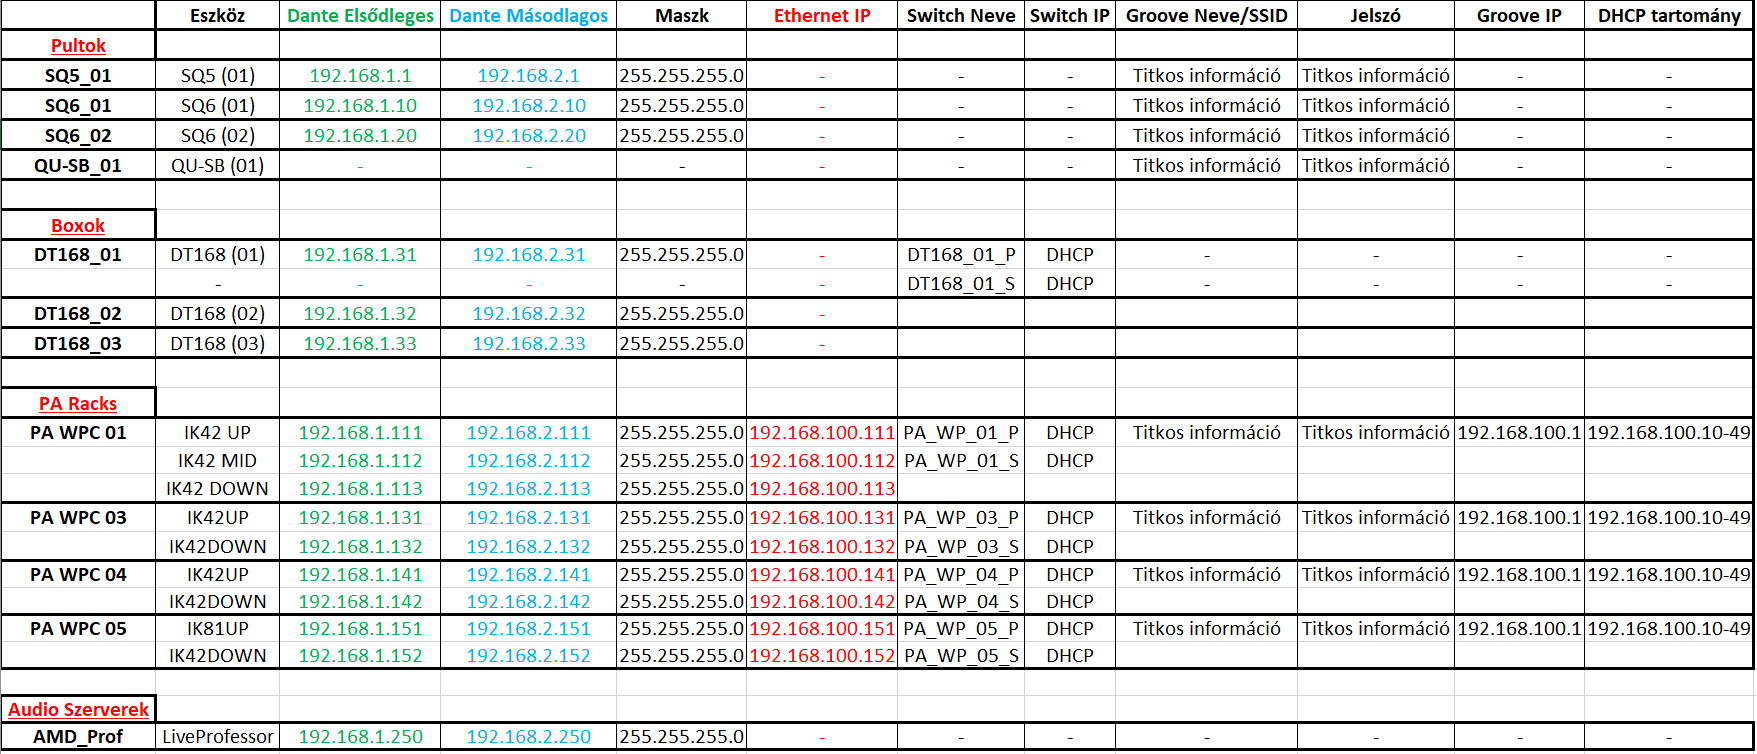
\includegraphics[width=\textwidth, keepaspectratio]{figures/dante_ips.png}
	\caption{Dante eszközök IP címei a hálózaton}\label{fig:dante_ips}
\end{figure}
%----------------------------------------------------------------------------
%----------------------------------------------------------------------------
\subsubsection{Dante Controller: Órajel nézet}
%----------------------------------------------------------------------------
Meg kell adnunk az audio hálózatunk master órajelét. Ehhez az órajelhez
szinkronizál a többi eszköz.
Az időszinkronizáció kulcsfontosságú élőzenei produkcióknál.
%----------------------------------------------------------------------------
\section{Rendszermérések és monitorozás}
%----------------------------------------------------------------------------
%----------------------------------------------------------------------------
\subsection{Dante rendszer monitorozása}
%----------------------------------------------------------------------------
%----------------------------------------------------------------------------
\subsubsection{Dante Controller: Hálózati állapot nézet}
%----------------------------------------------------------------------------
%----------------------------------------------------------------------------
\subsubsection{Dante Controller: Események nézet}
%----------------------------------------------------------------------------
%----------------------------------------------------------------------------
\subsection{Cardioid mélyláda rendszer mérése}
%----------------------------------------------------------------------------
%----------------------------------------------------------------------------
\subsection{Mélyláda és Line Array fázishelyesség}
%----------------------------------------------------------------------------
%----------------------------------------------------------------------------
\subsection{Rendszer hangnyomás szint és frekvencia átvitel mérése}
%----------------------------------------------------------------------------